\documentclass[openany]{book}
\usepackage{lmodern}
\usepackage{amssymb,amsmath}
\usepackage{ifxetex,ifluatex}
\usepackage{fixltx2e} % provides \textsubscript
\ifnum 0\ifxetex 1\fi\ifluatex 1\fi=0 % if pdftex
  \usepackage[T1]{fontenc}
  \usepackage[utf8]{inputenc}
\else % if luatex or xelatex
  \ifxetex
    \usepackage{mathspec}
  \else
    \usepackage{fontspec}
  \fi
  \defaultfontfeatures{Ligatures=TeX,Scale=MatchLowercase}
\fi
% use upquote if available, for straight quotes in verbatim environments
\IfFileExists{upquote.sty}{\usepackage{upquote}}{}
% use microtype if available
\IfFileExists{microtype.sty}{%
\usepackage{microtype}
\UseMicrotypeSet[protrusion]{basicmath} % disable protrusion for tt fonts
}{}
\usepackage[margin=1in]{geometry}
\usepackage{hyperref}
\hypersetup{unicode=true,
            pdftitle={结直肠癌差异甲基化区域~},
            pdfauthor={~; 艾米森生命科技有限公司; 生物信息部; ~},
            pdfborder={0 0 0},
            breaklinks=true}
\urlstyle{same}  % don't use monospace font for urls
\usepackage{natbib}
\bibliographystyle{apalike}
\usepackage{longtable,booktabs}
\usepackage{graphicx,grffile}
\makeatletter
\def\maxwidth{\ifdim\Gin@nat@width>\linewidth\linewidth\else\Gin@nat@width\fi}
\def\maxheight{\ifdim\Gin@nat@height>\textheight\textheight\else\Gin@nat@height\fi}
\makeatother
% Scale images if necessary, so that they will not overflow the page
% margins by default, and it is still possible to overwrite the defaults
% using explicit options in \includegraphics[width, height, ...]{}
\setkeys{Gin}{width=\maxwidth,height=\maxheight,keepaspectratio}
\IfFileExists{parskip.sty}{%
\usepackage{parskip}
}{% else
\setlength{\parindent}{0pt}
\setlength{\parskip}{6pt plus 2pt minus 1pt}
}
\setlength{\emergencystretch}{3em}  % prevent overfull lines
\providecommand{\tightlist}{%
  \setlength{\itemsep}{0pt}\setlength{\parskip}{0pt}}
\setcounter{secnumdepth}{5}
% Redefines (sub)paragraphs to behave more like sections
\ifx\paragraph\undefined\else
\let\oldparagraph\paragraph
\renewcommand{\paragraph}[1]{\oldparagraph{#1}\mbox{}}
\fi
\ifx\subparagraph\undefined\else
\let\oldsubparagraph\subparagraph
\renewcommand{\subparagraph}[1]{\oldsubparagraph{#1}\mbox{}}
\fi

%%% Use protect on footnotes to avoid problems with footnotes in titles
\let\rmarkdownfootnote\footnote%
\def\footnote{\protect\rmarkdownfootnote}

%%% Change title format to be more compact
\usepackage{titling}

% Create subtitle command for use in maketitle
\providecommand{\subtitle}[1]{
  \posttitle{
    \begin{center}\large#1\end{center}
    }
}

\setlength{\droptitle}{-2em}

  \title{结直肠癌差异甲基化区域~}
    \pretitle{\vspace{\droptitle}\centering\huge}
  \posttitle{\par}
    \author{~ \\ 艾米森生命科技有限公司 \\ 生物信息部 \\ ~}
    \preauthor{\centering\large\emph}
  \postauthor{\par}
      \predate{\centering\large\emph}
  \postdate{\par}
    \date{2019-05-27}

\usepackage{booktabs}
\usepackage{xeCJK}
\setCJKmainfont{simsun.ttc}
\usepackage[table]{xcolor}

\begin{document}
\maketitle

{
\setcounter{tocdepth}{1}
\tableofcontents
}
\chapter{问题描述}

SDC2 三个DMR的序列和位置已经发给您,烦请补充以下结果:
首先,将390多例癌症样本按照部位进行分类(如直肠、乙状结肠、升结肠等等)
对于每个部位的癌症,做6条ROC曲线,分别是单个DMR的ROC和两个DMR
组合的ROC,各三个。 谢谢!

\chapter{解决方案}

\section{思路}

TCGA结直肠癌数据集共包含387个病人,总计438例样本,其中癌症样本393例,癌旁45例.
查阅临床信息,整理各个部位的样本分布列表如下:

\begin{table}[!h]

\caption{\label{tab:example}结直肠各部位样本数}
\centering
\begin{tabular}{llr}
\toprule
部位 & 样本类别 & 样本数量\\
\midrule
\rowcolor{gray!6}  Cecum & cancer & 71\\
Cecum & normal & 7\\
\rowcolor{gray!6}  Sigmoid colon & cancer & 67\\
Sigmoid colon & normal & 7\\
\rowcolor{gray!6}  Ascending colon & cancer & 60\\
\addlinespace
Ascending colon & normal & 6\\
\rowcolor{gray!6}  Colon, NOS & cancer & 49\\
Colon, NOS & normal & 12\\
\rowcolor{gray!6}  Rectum, NOS & cancer & 49\\
Rectum, NOS & normal & 6\\
\addlinespace
\rowcolor{gray!6}  Rectosigmoid junction & cancer & 46\\
Rectosigmoid junction & normal & 2\\
\rowcolor{gray!6}  Descending colon & cancer & 14\\
Descending colon & normal & 2\\
\rowcolor{gray!6}  Hepatic flexure of colon & cancer & 13\\
\addlinespace
Hepatic flexure of colon & normal & 3\\
\rowcolor{gray!6}  Transverse colon & cancer & 14\\
Splenic flexure of colon & cancer & 5\\
\rowcolor{gray!6}  -- & cancer & 3\\
Connective, subcutaneous and other soft tissues of abdomen & cancer & 2\\
\bottomrule
\end{tabular}
\end{table}

从上表可见,大多数部位的癌旁样本非常少。为此,我们将所有45例癌旁样本当作一个整体,与其它各个部位的癌症样本进行比较分析,做出ROC曲线。
根据你提供的序列,我们找到对应的三个DMR区域的探针构成如下:

\begin{itemize}
\tightlist
\item
  DMR1: cg13096260; cg18719750; cg24732574; cg08979737; cg25070637
\item
  DMR2: cg08979737; cg25070637; cg14538332; cg16935295
\item
  DMR3: cg14538332; cg16935295
\end{itemize}

对于一个样本来说,我们采用该样本在这个DMR上的所有探针的甲基化水平的均值,作为该样本在这个DMR上的甲基化水平。如果两个或两个以上DMR组合使用,我们分别求出该样本在不同DMR上的甲基化水平,然后用random
forest模型进行建模,获得该模型的ROC曲线。

Cecum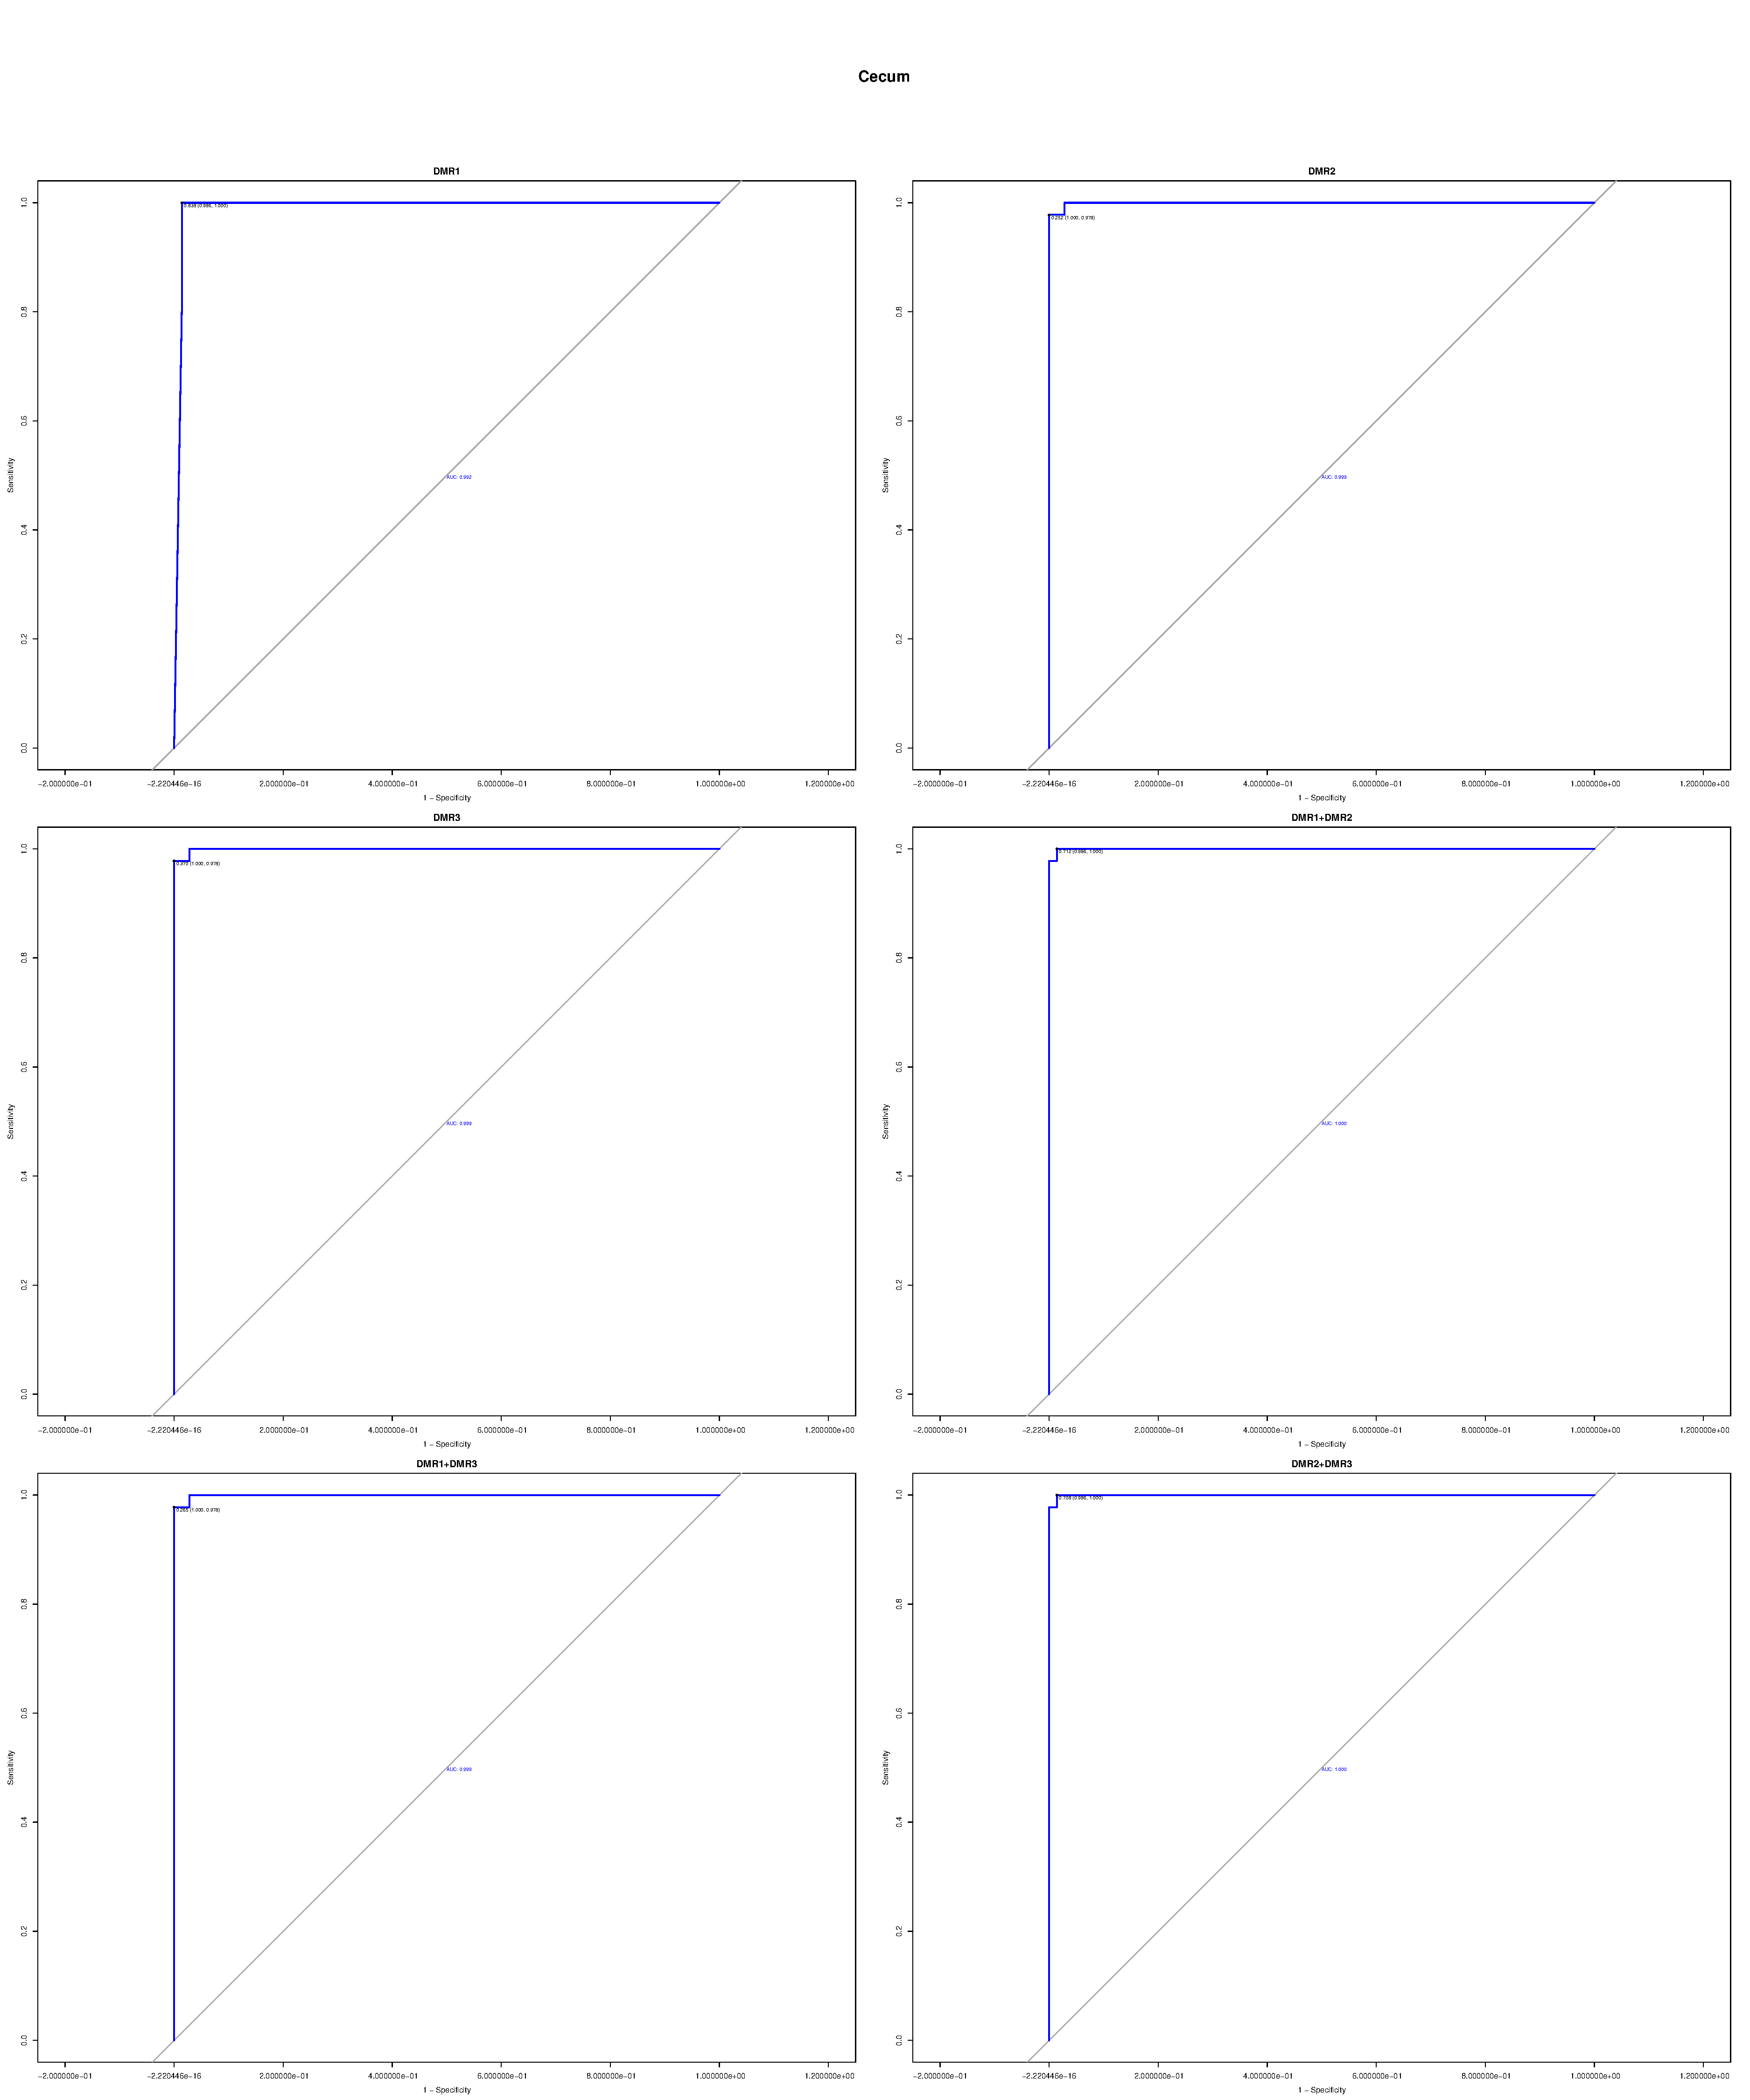
\includegraphics{book1_files/figure-latex/plots-1.pdf} Sigmoid
colon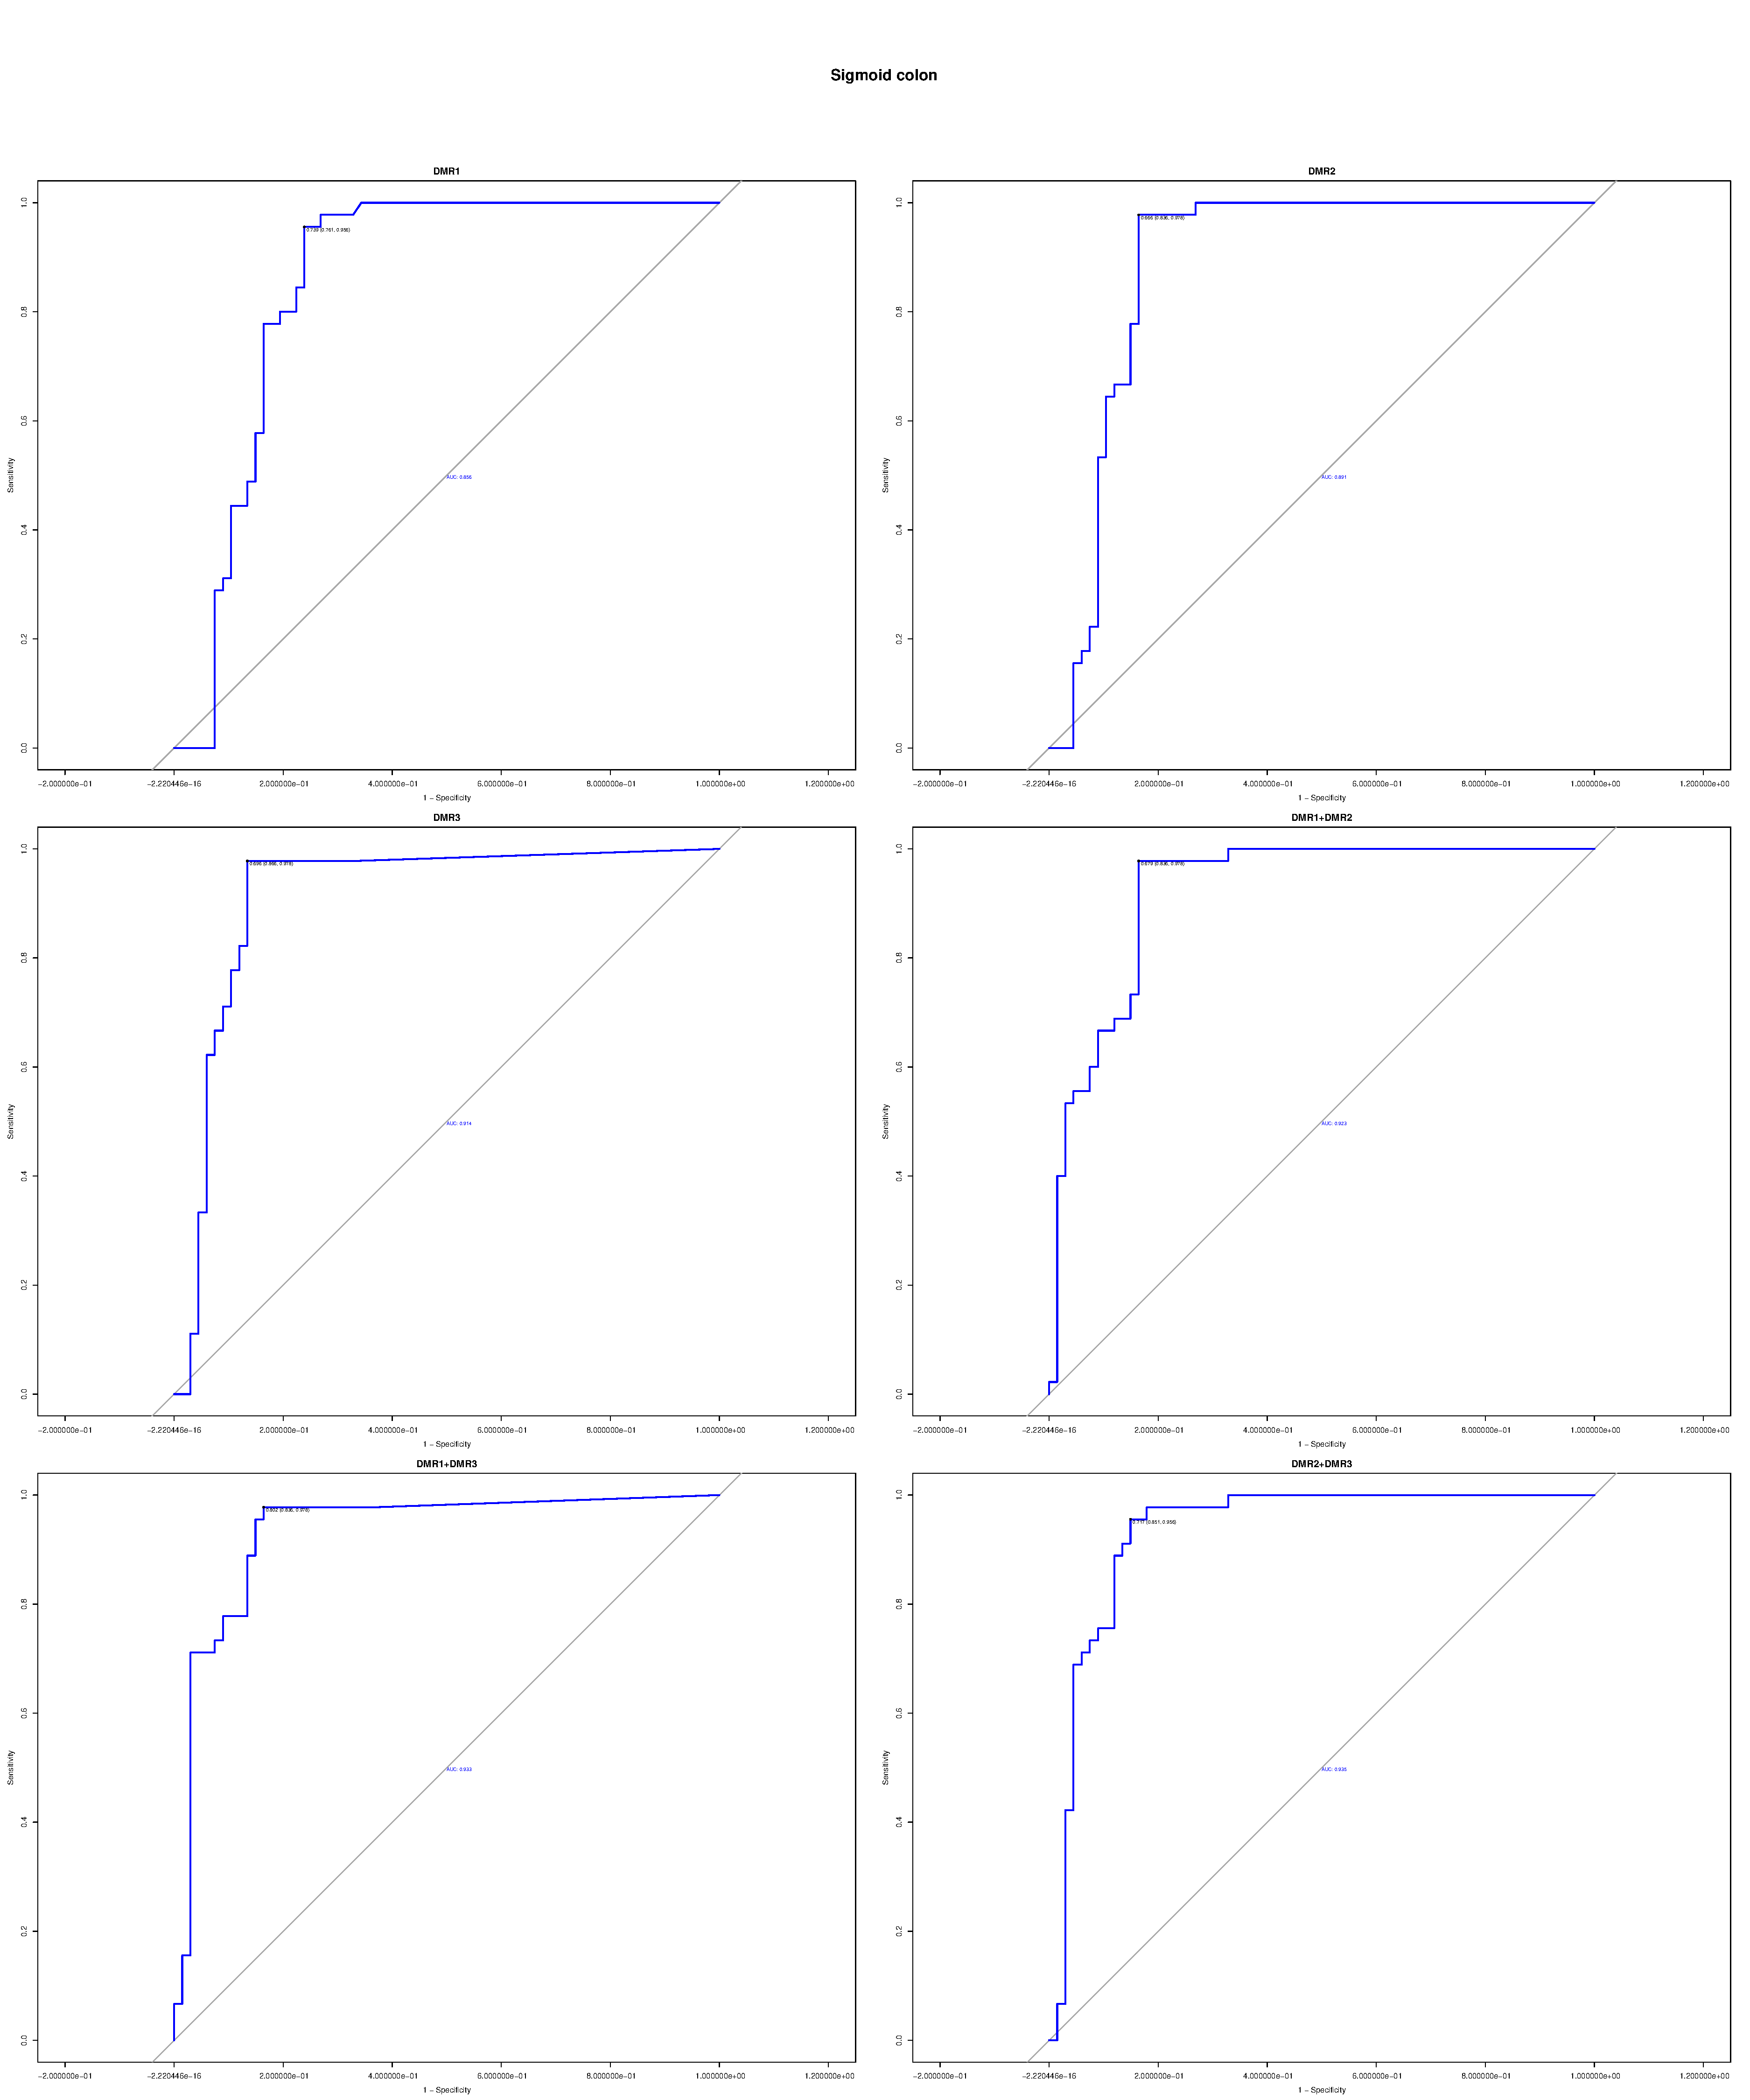
\includegraphics{book1_files/figure-latex/plots-2.pdf} Ascending
colon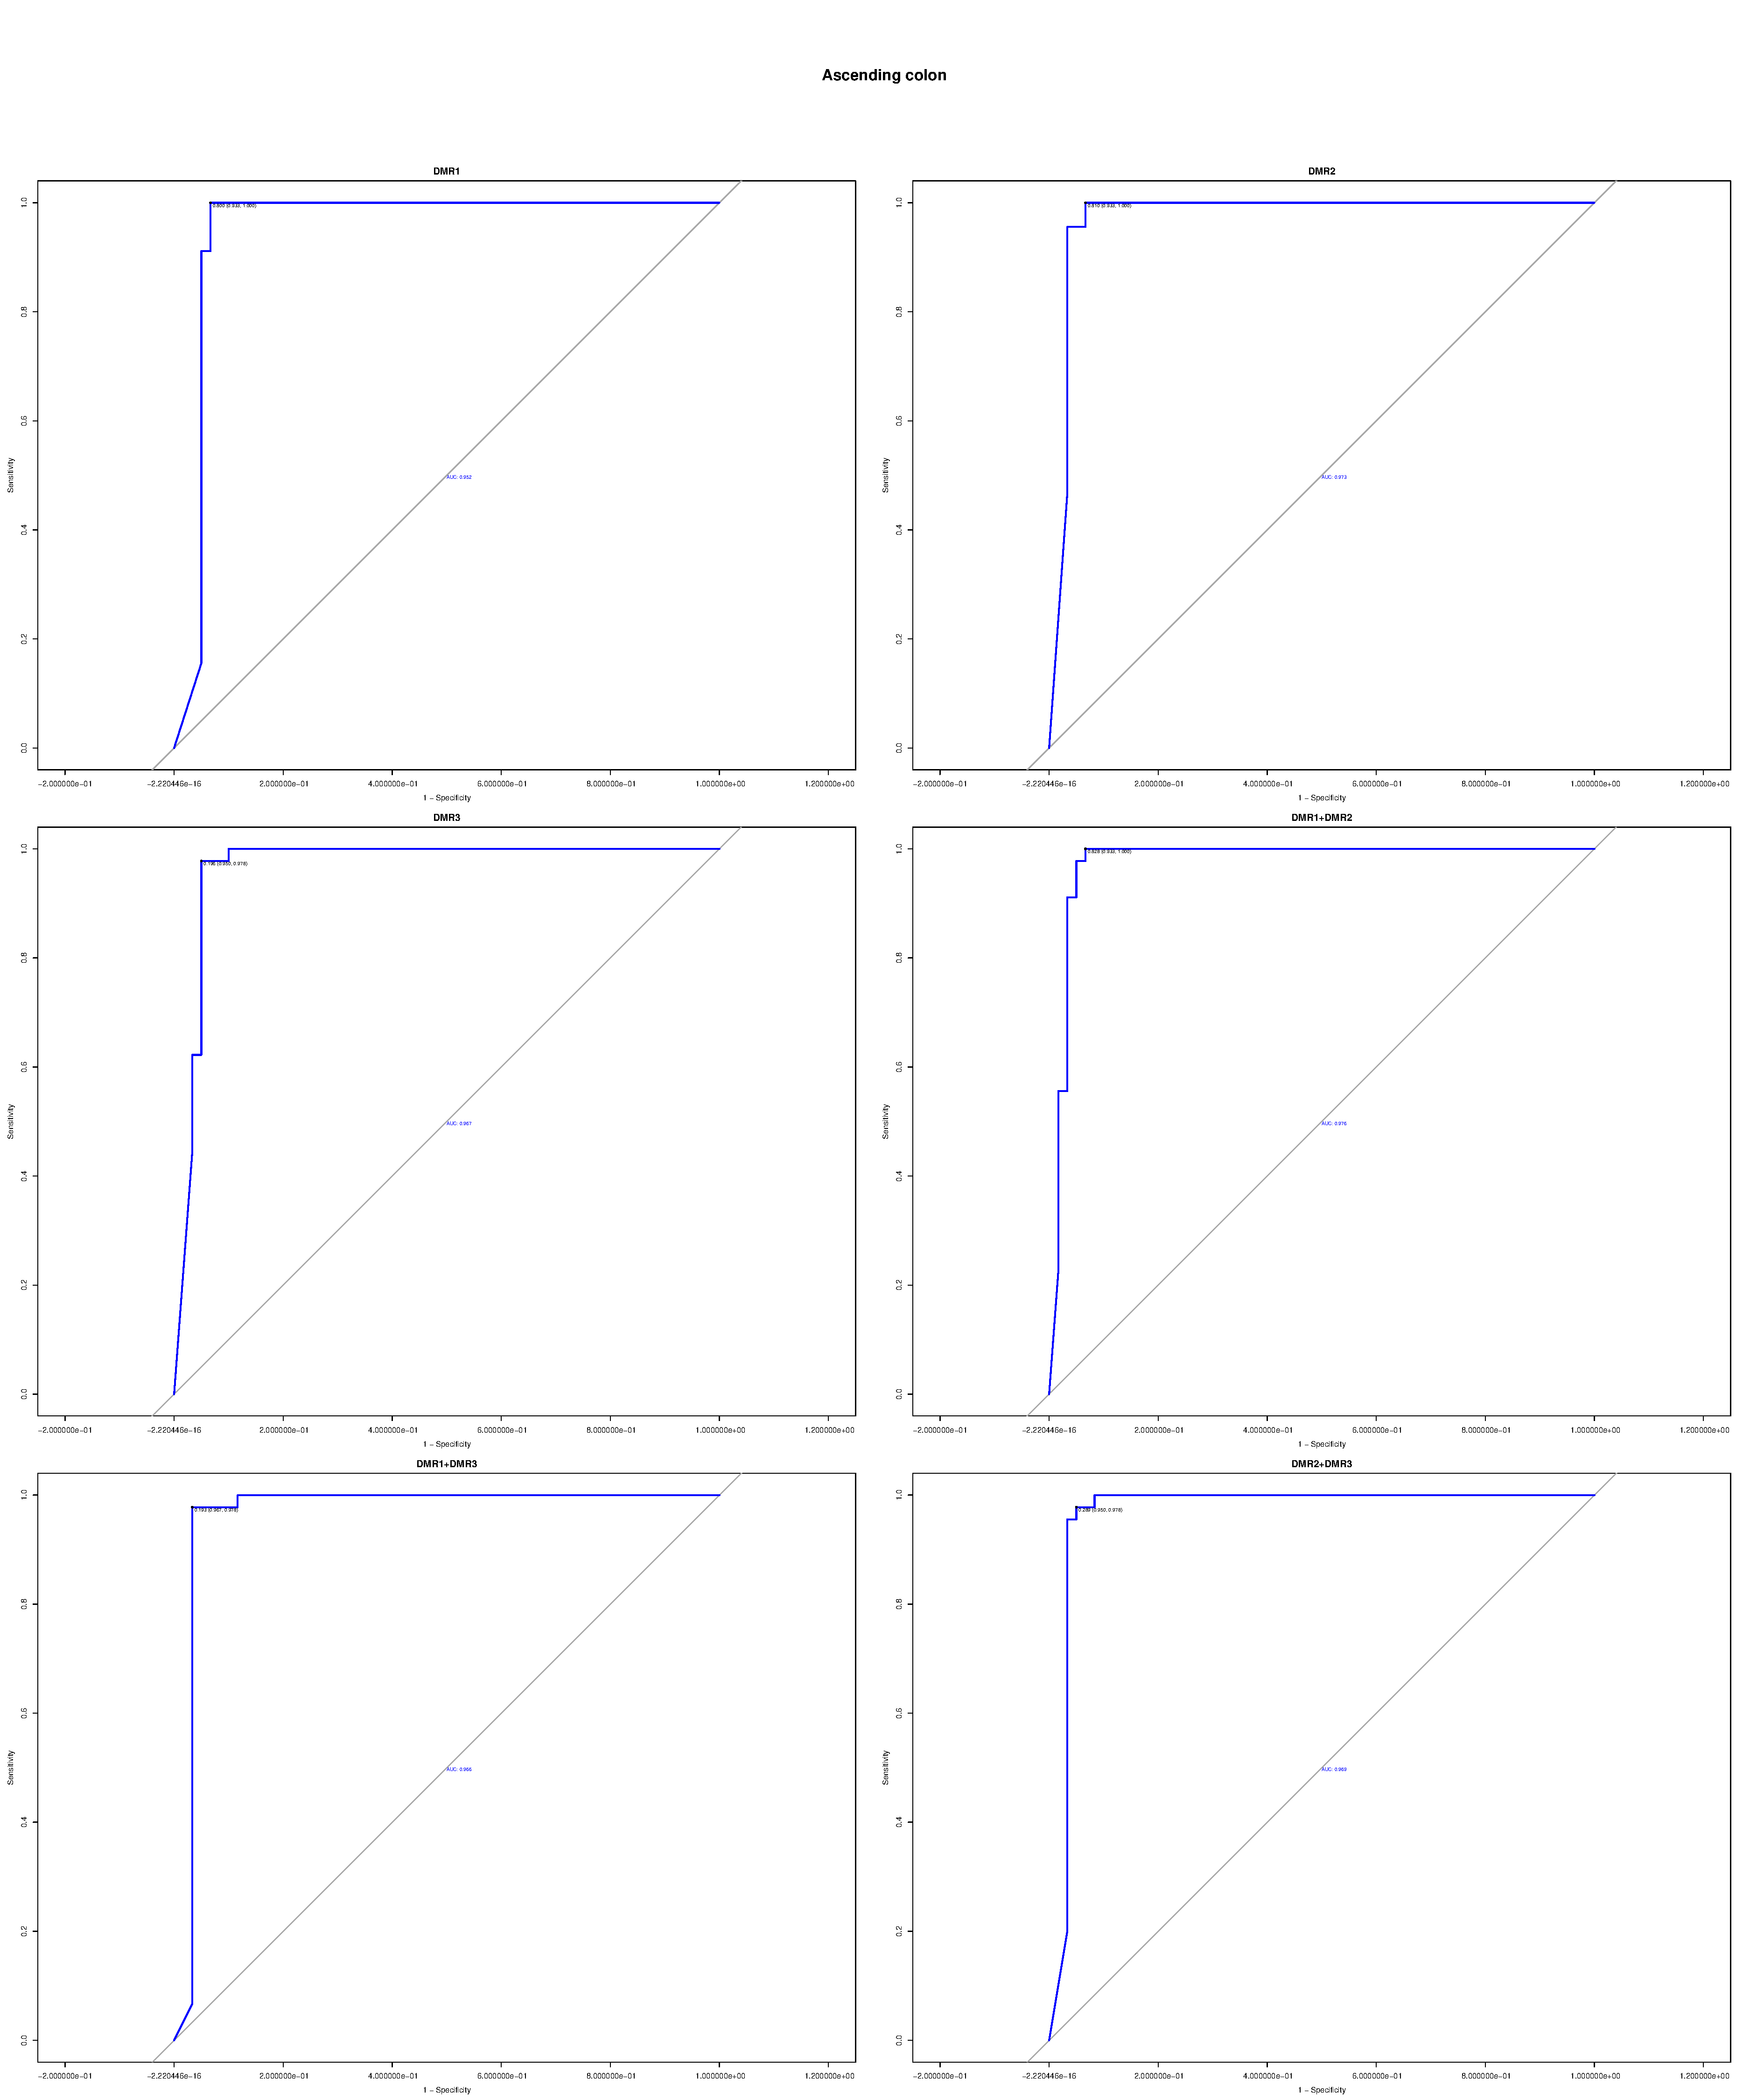
\includegraphics{book1_files/figure-latex/plots-3.pdf} Colon,
NOS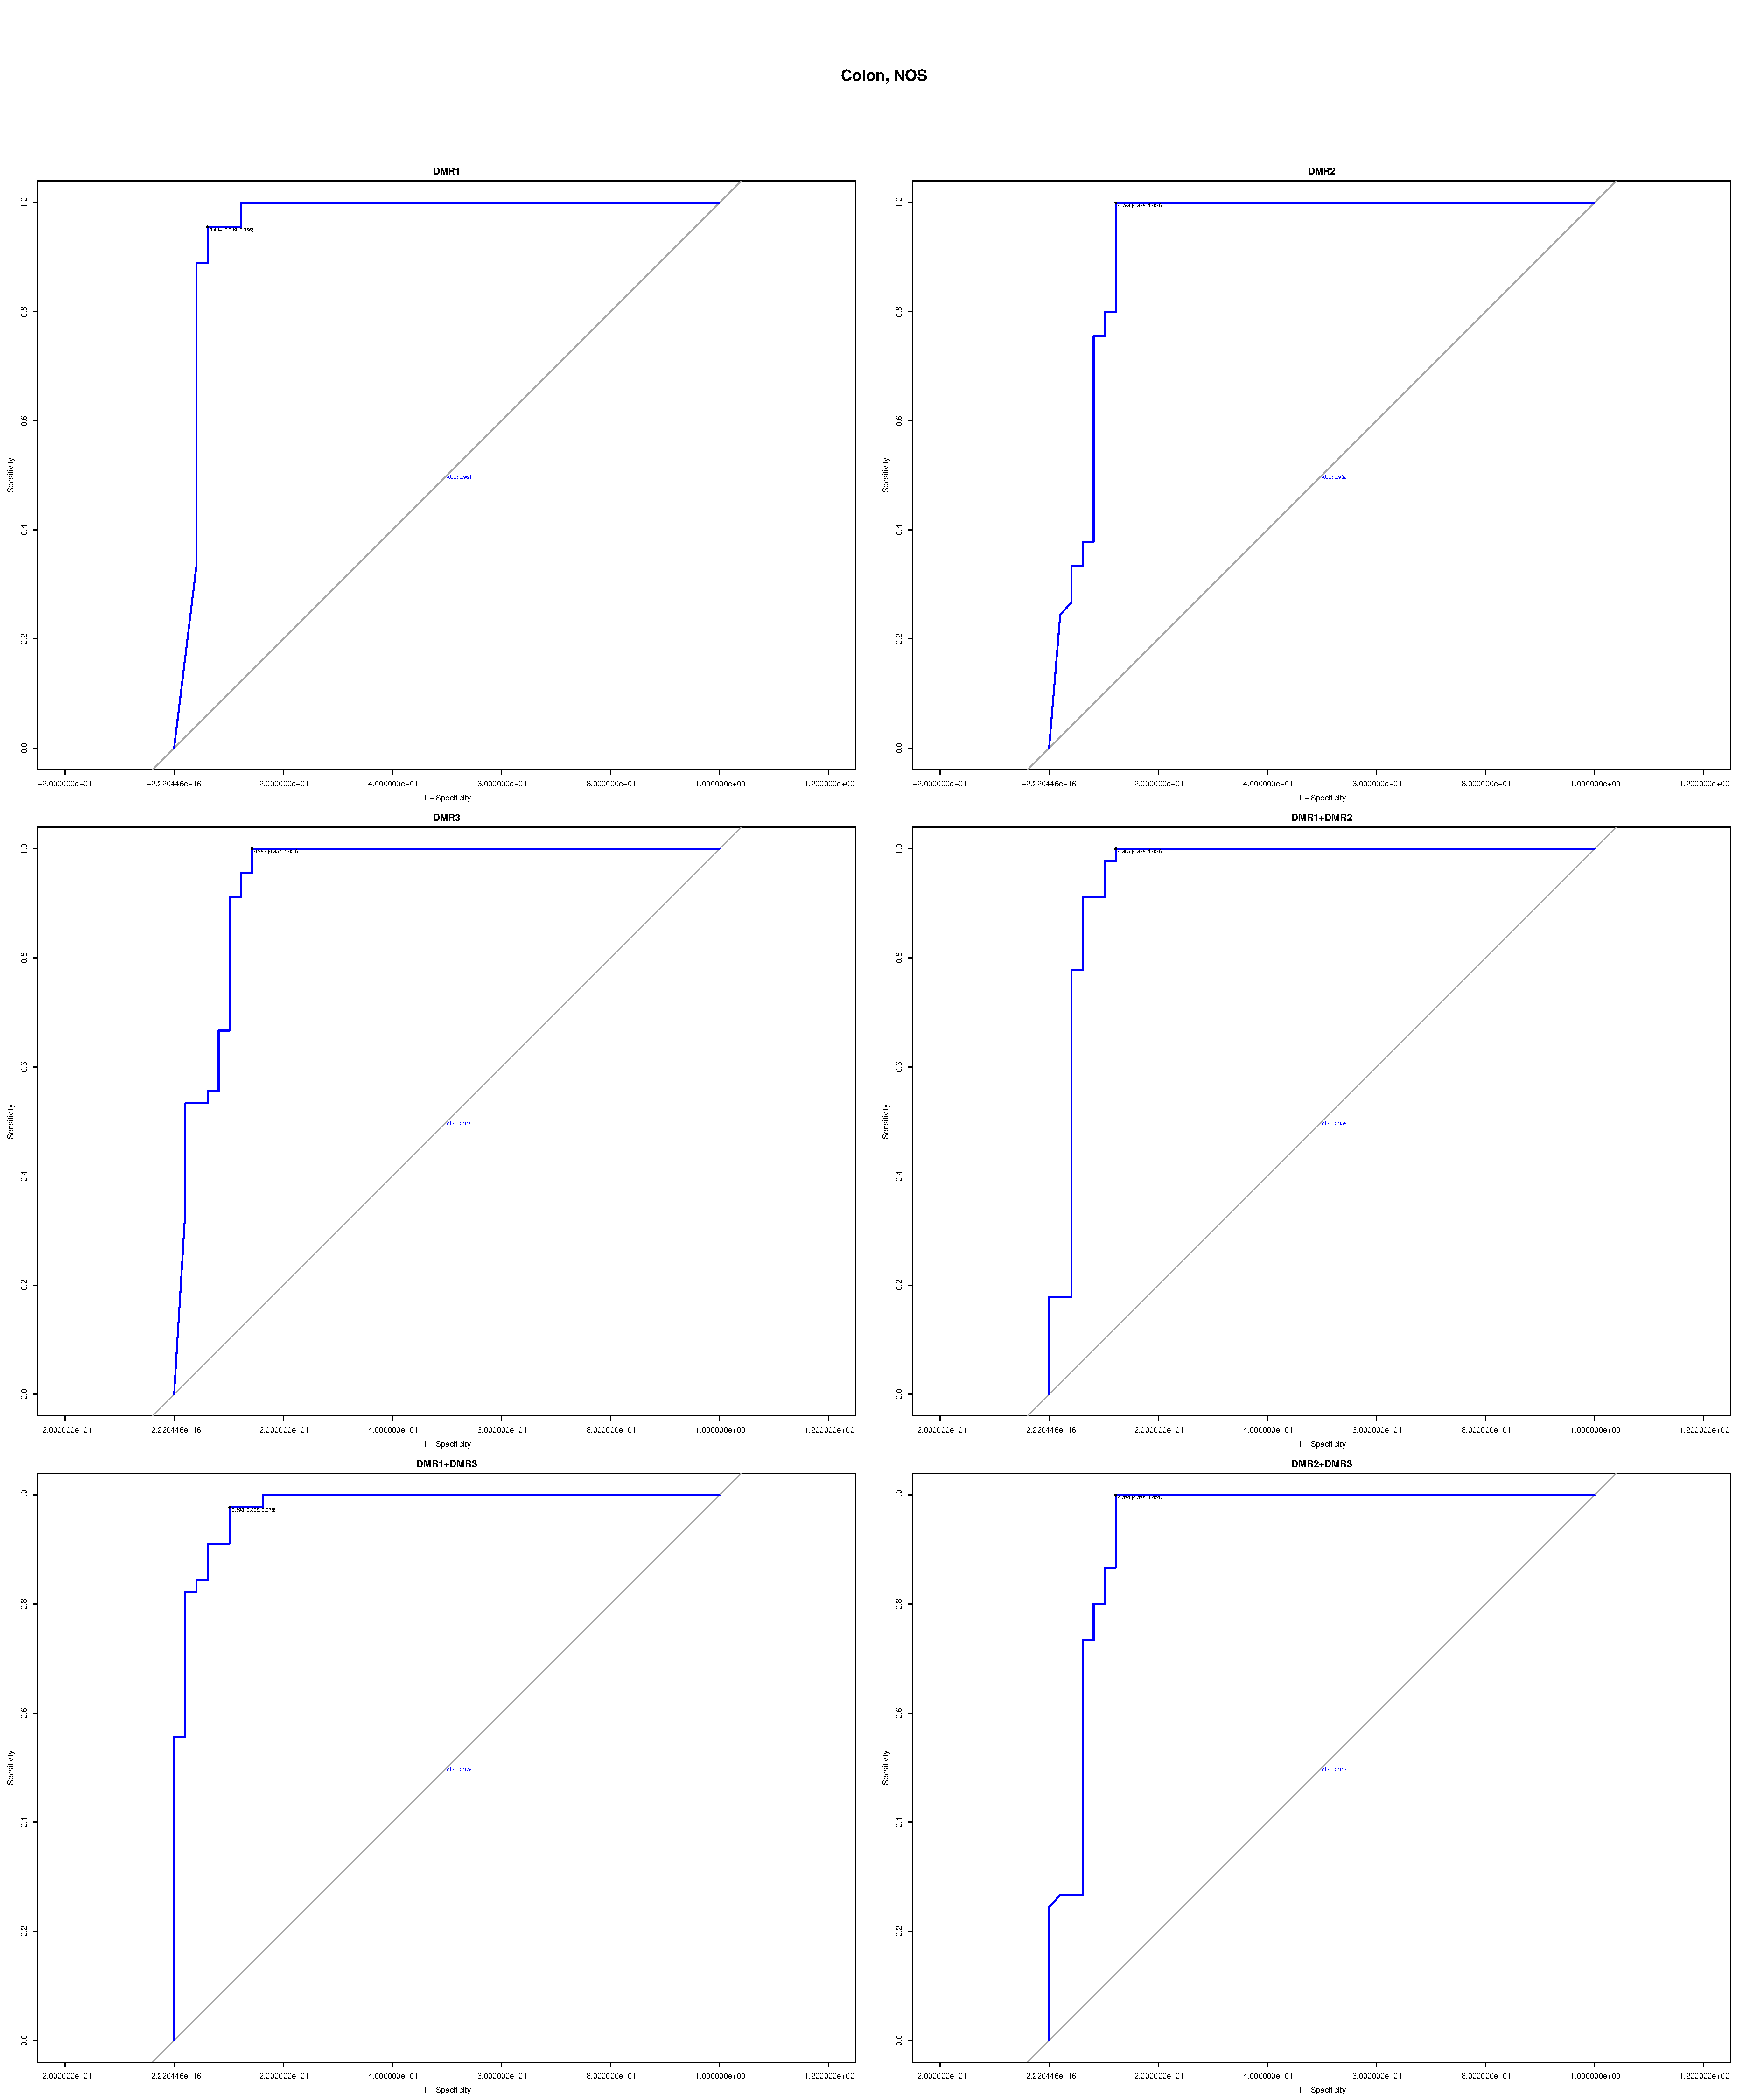
\includegraphics{book1_files/figure-latex/plots-4.pdf} Rectum,
NOS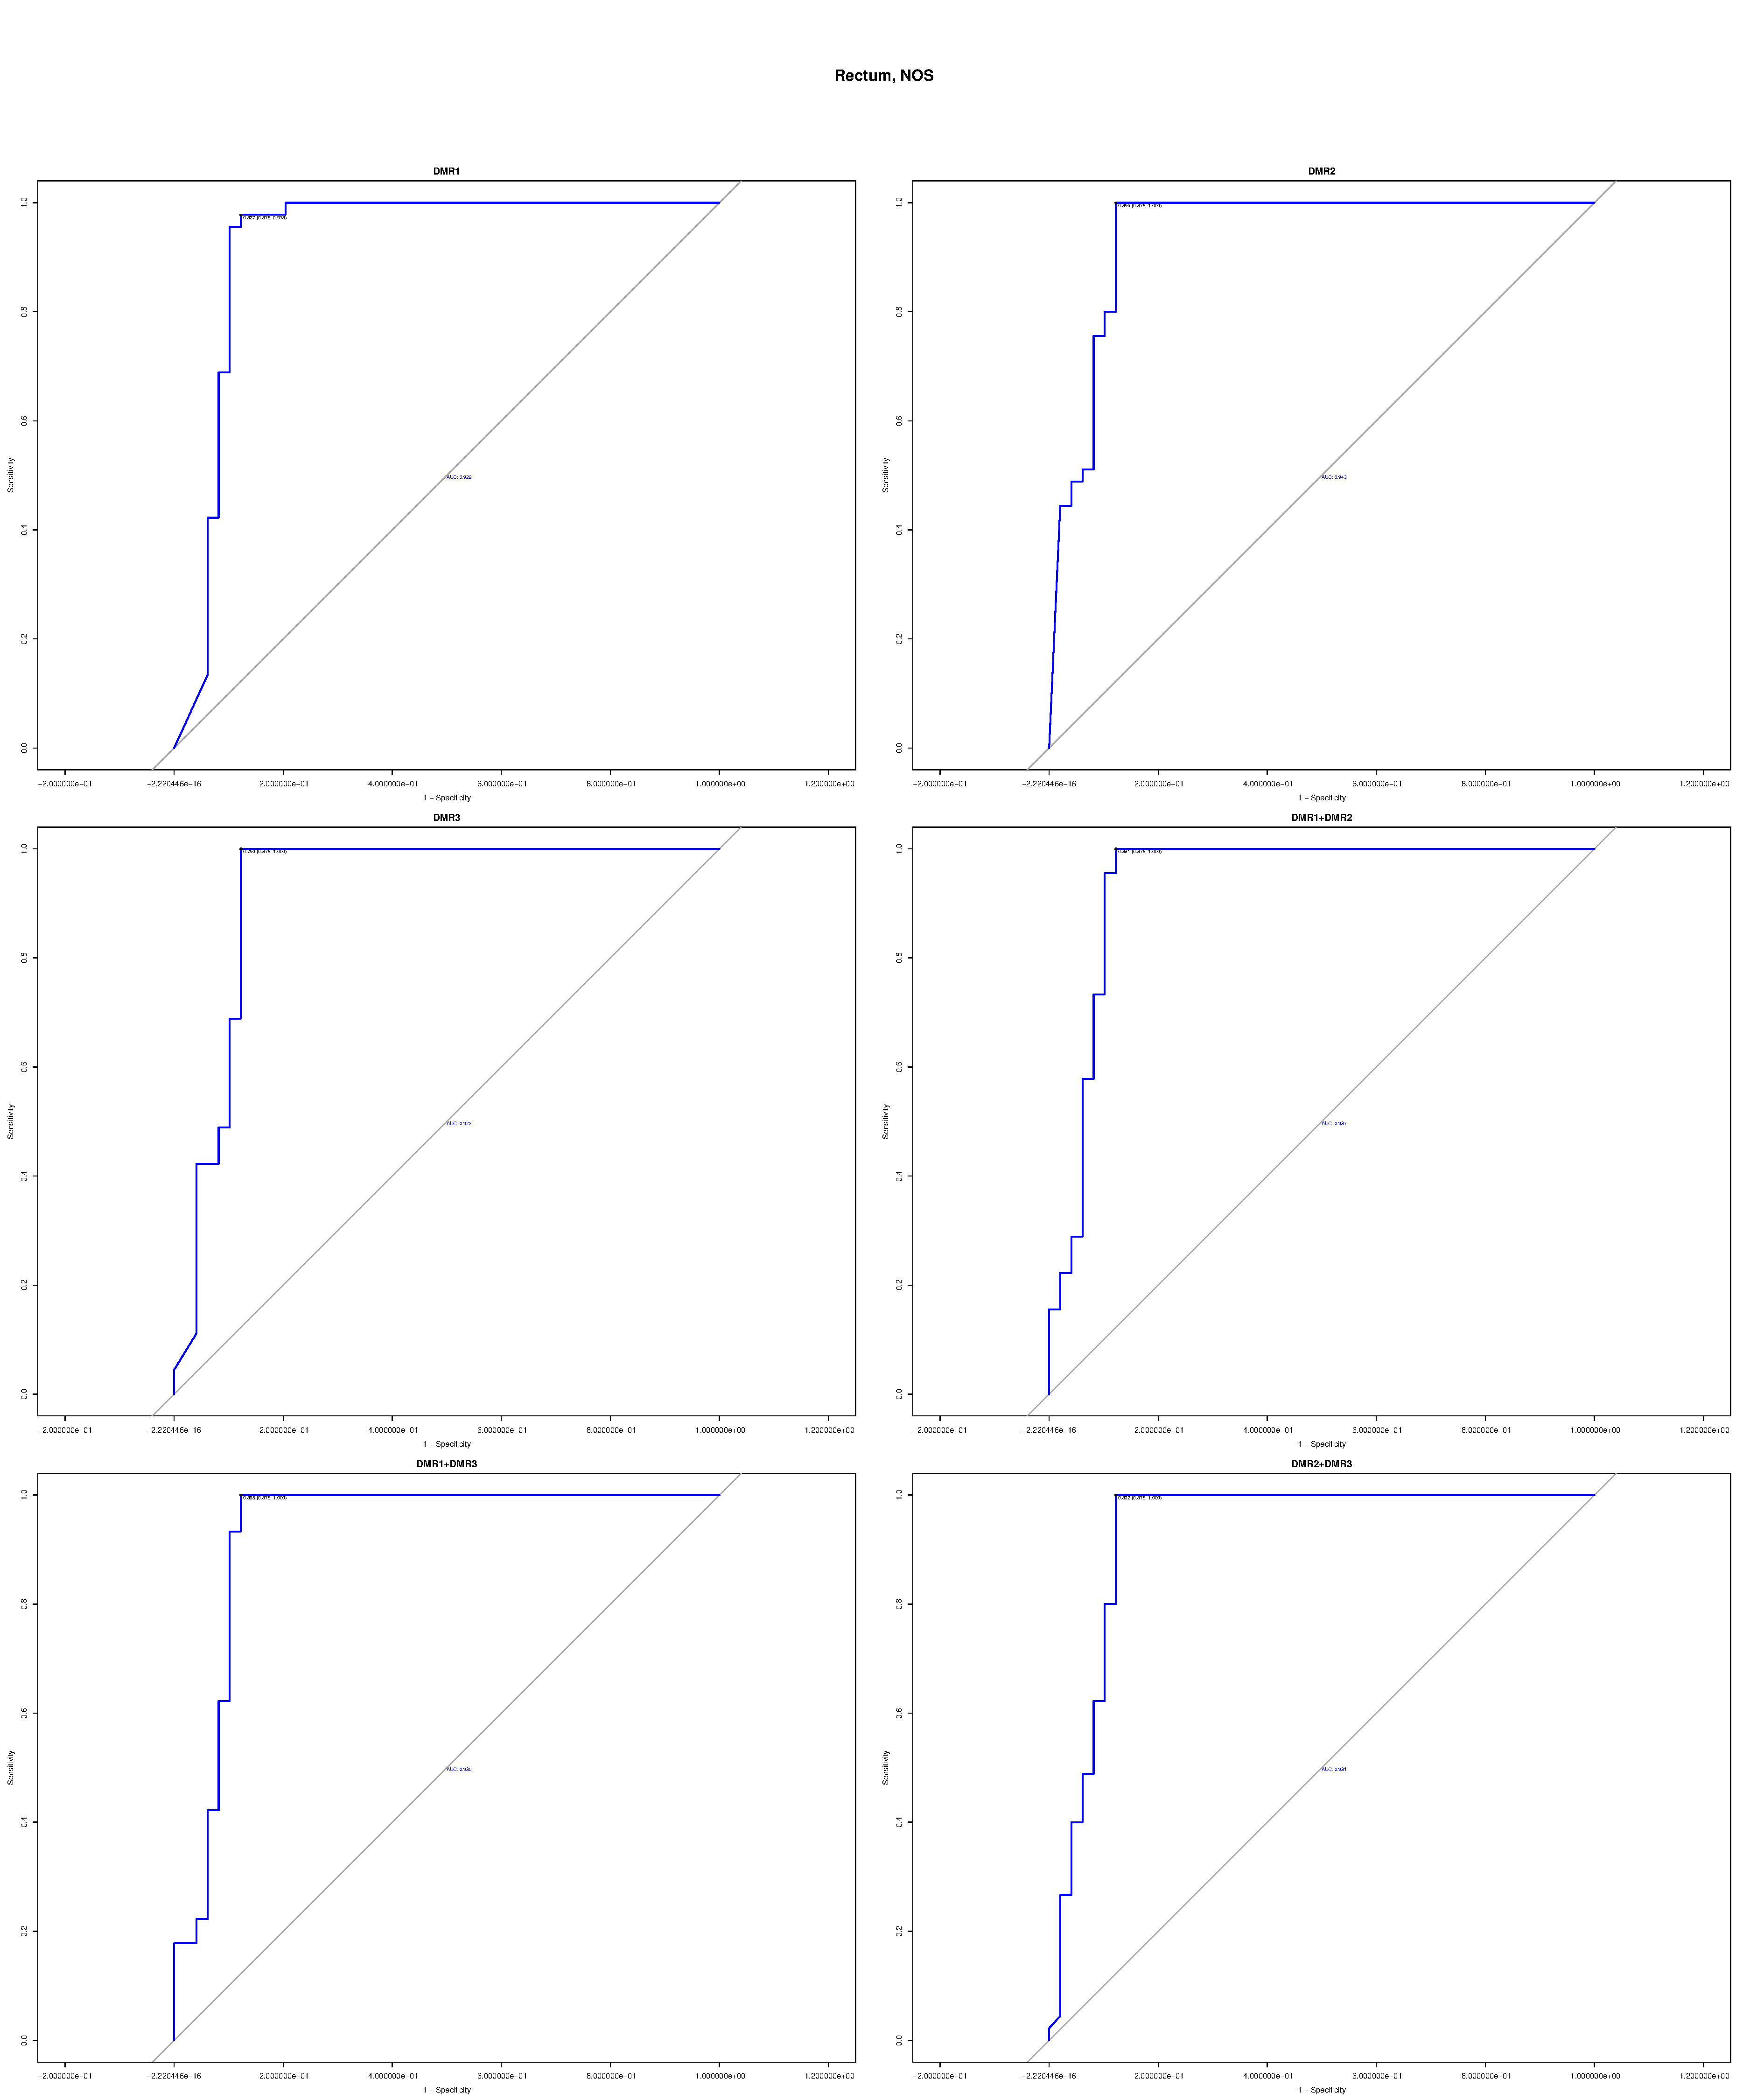
\includegraphics{book1_files/figure-latex/plots-5.pdf} Rectosigmoid
junction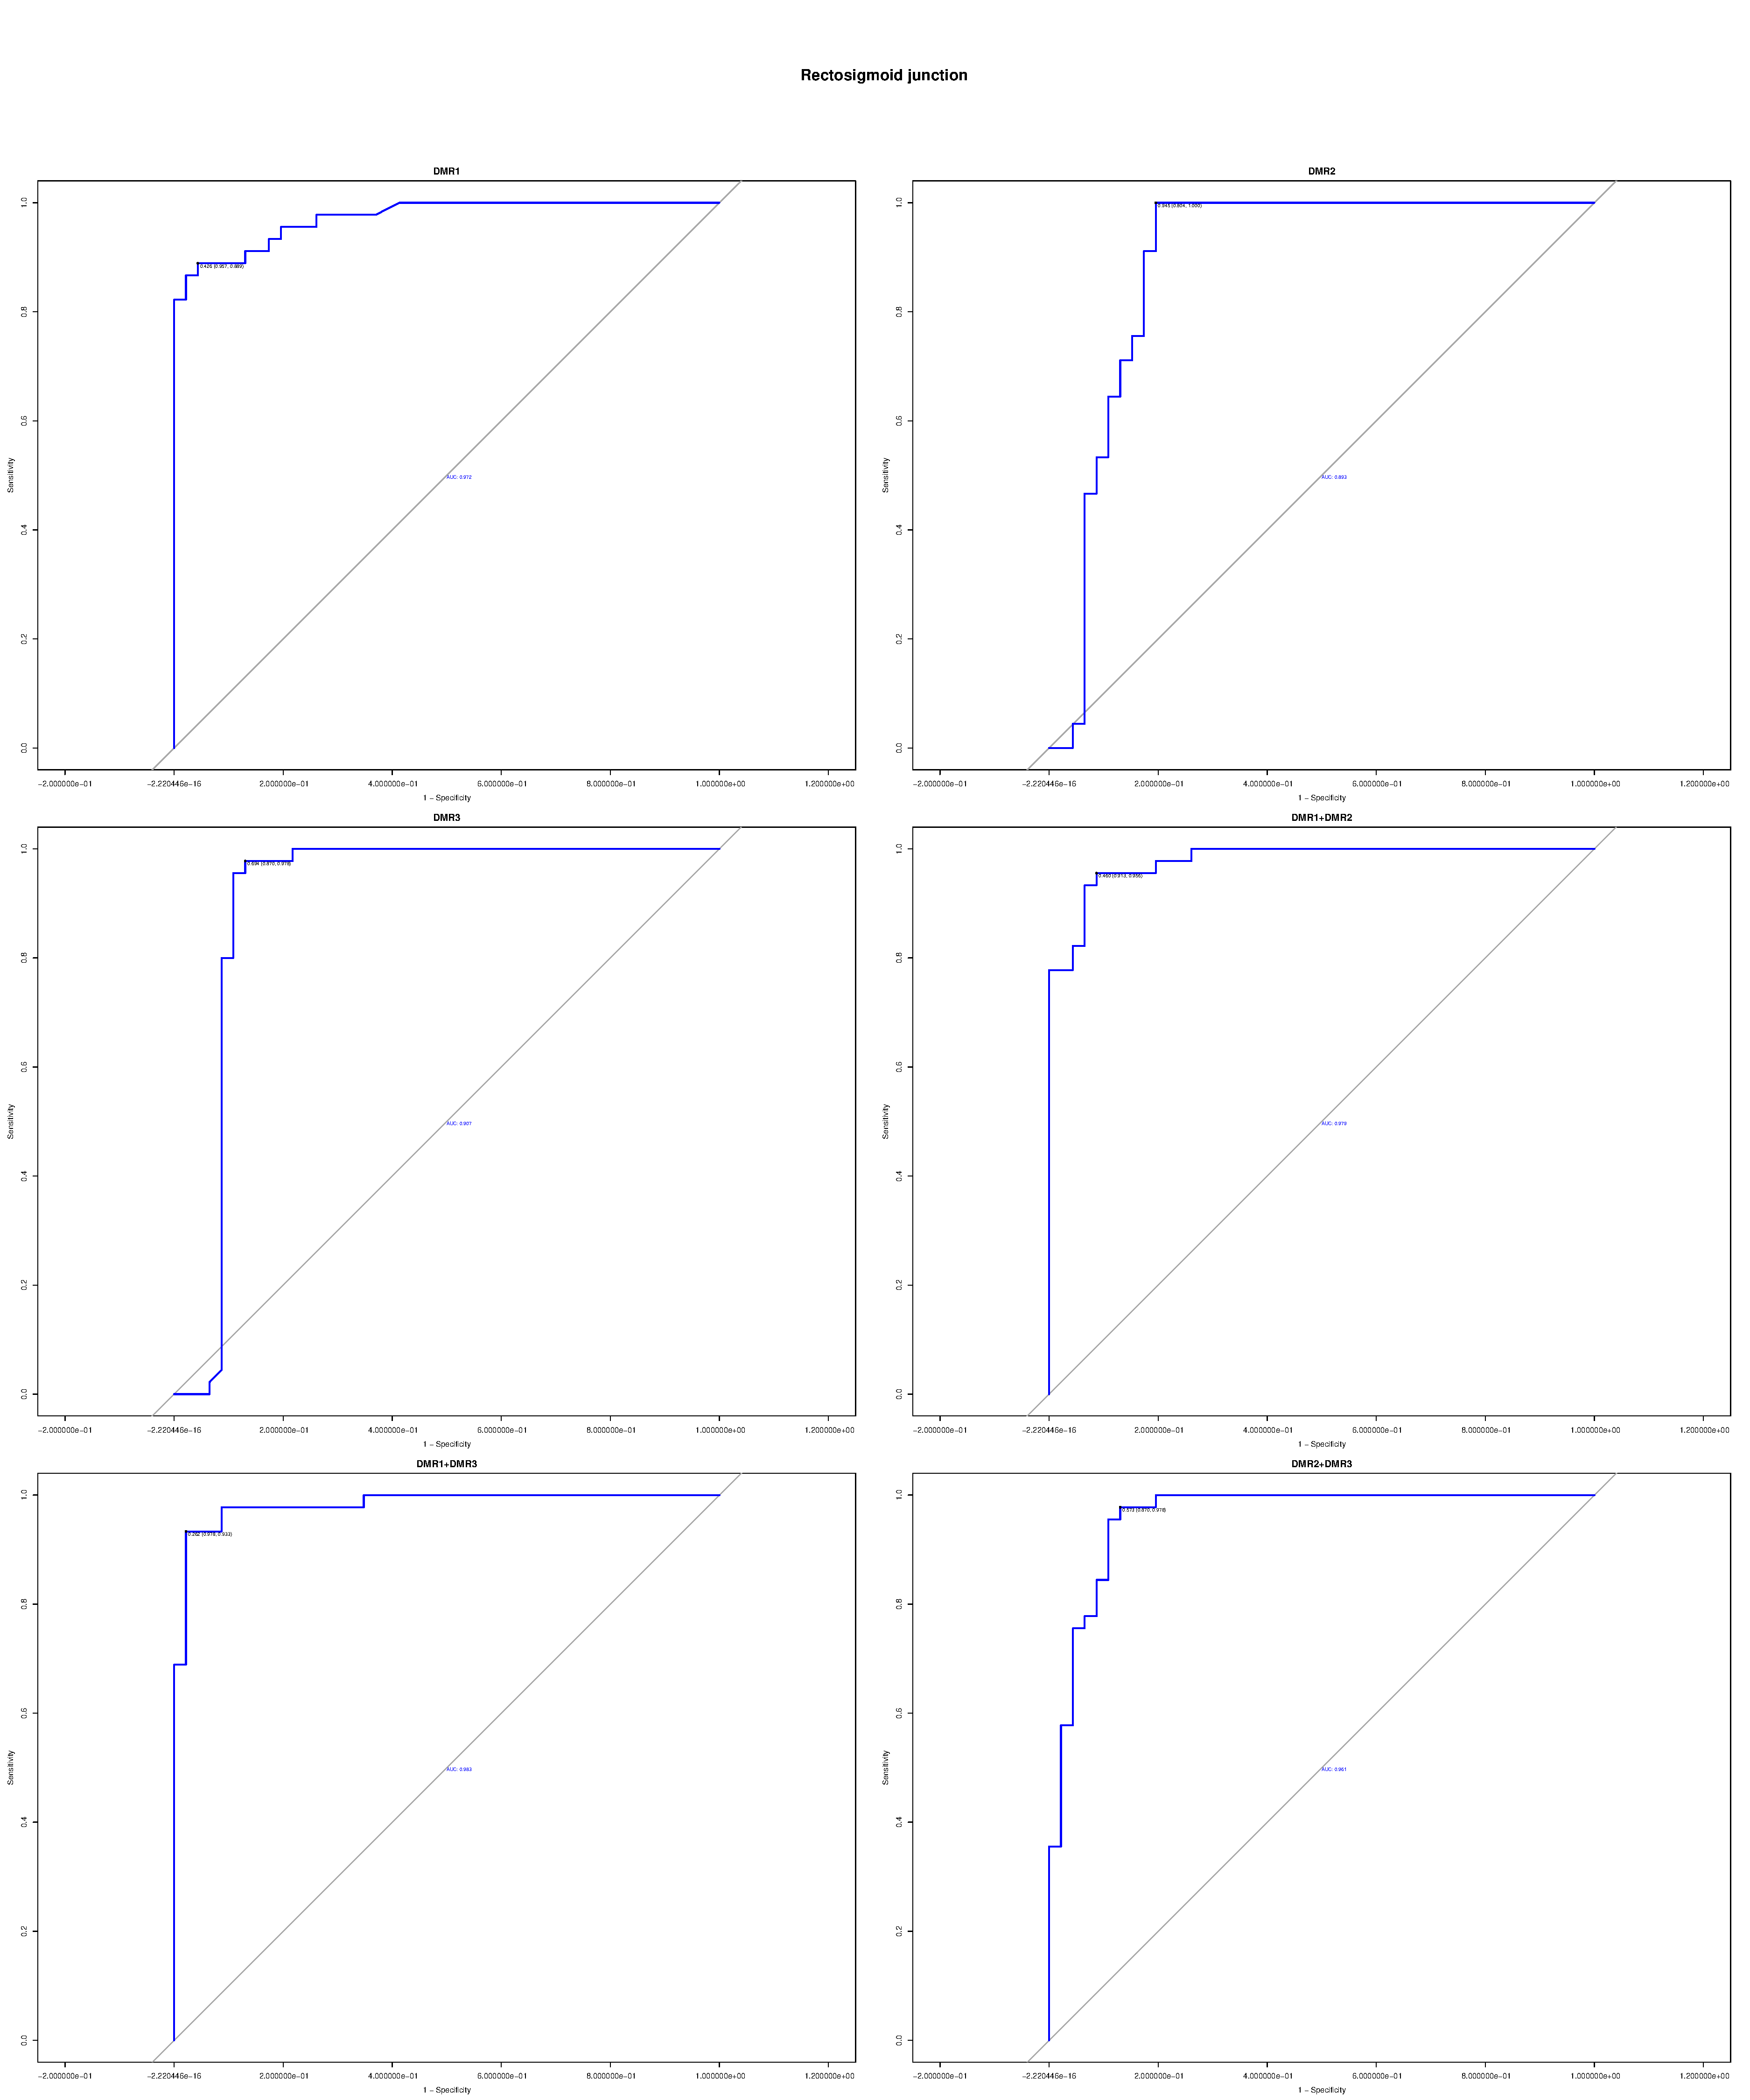
\includegraphics{book1_files/figure-latex/plots-6.pdf}
Descending colon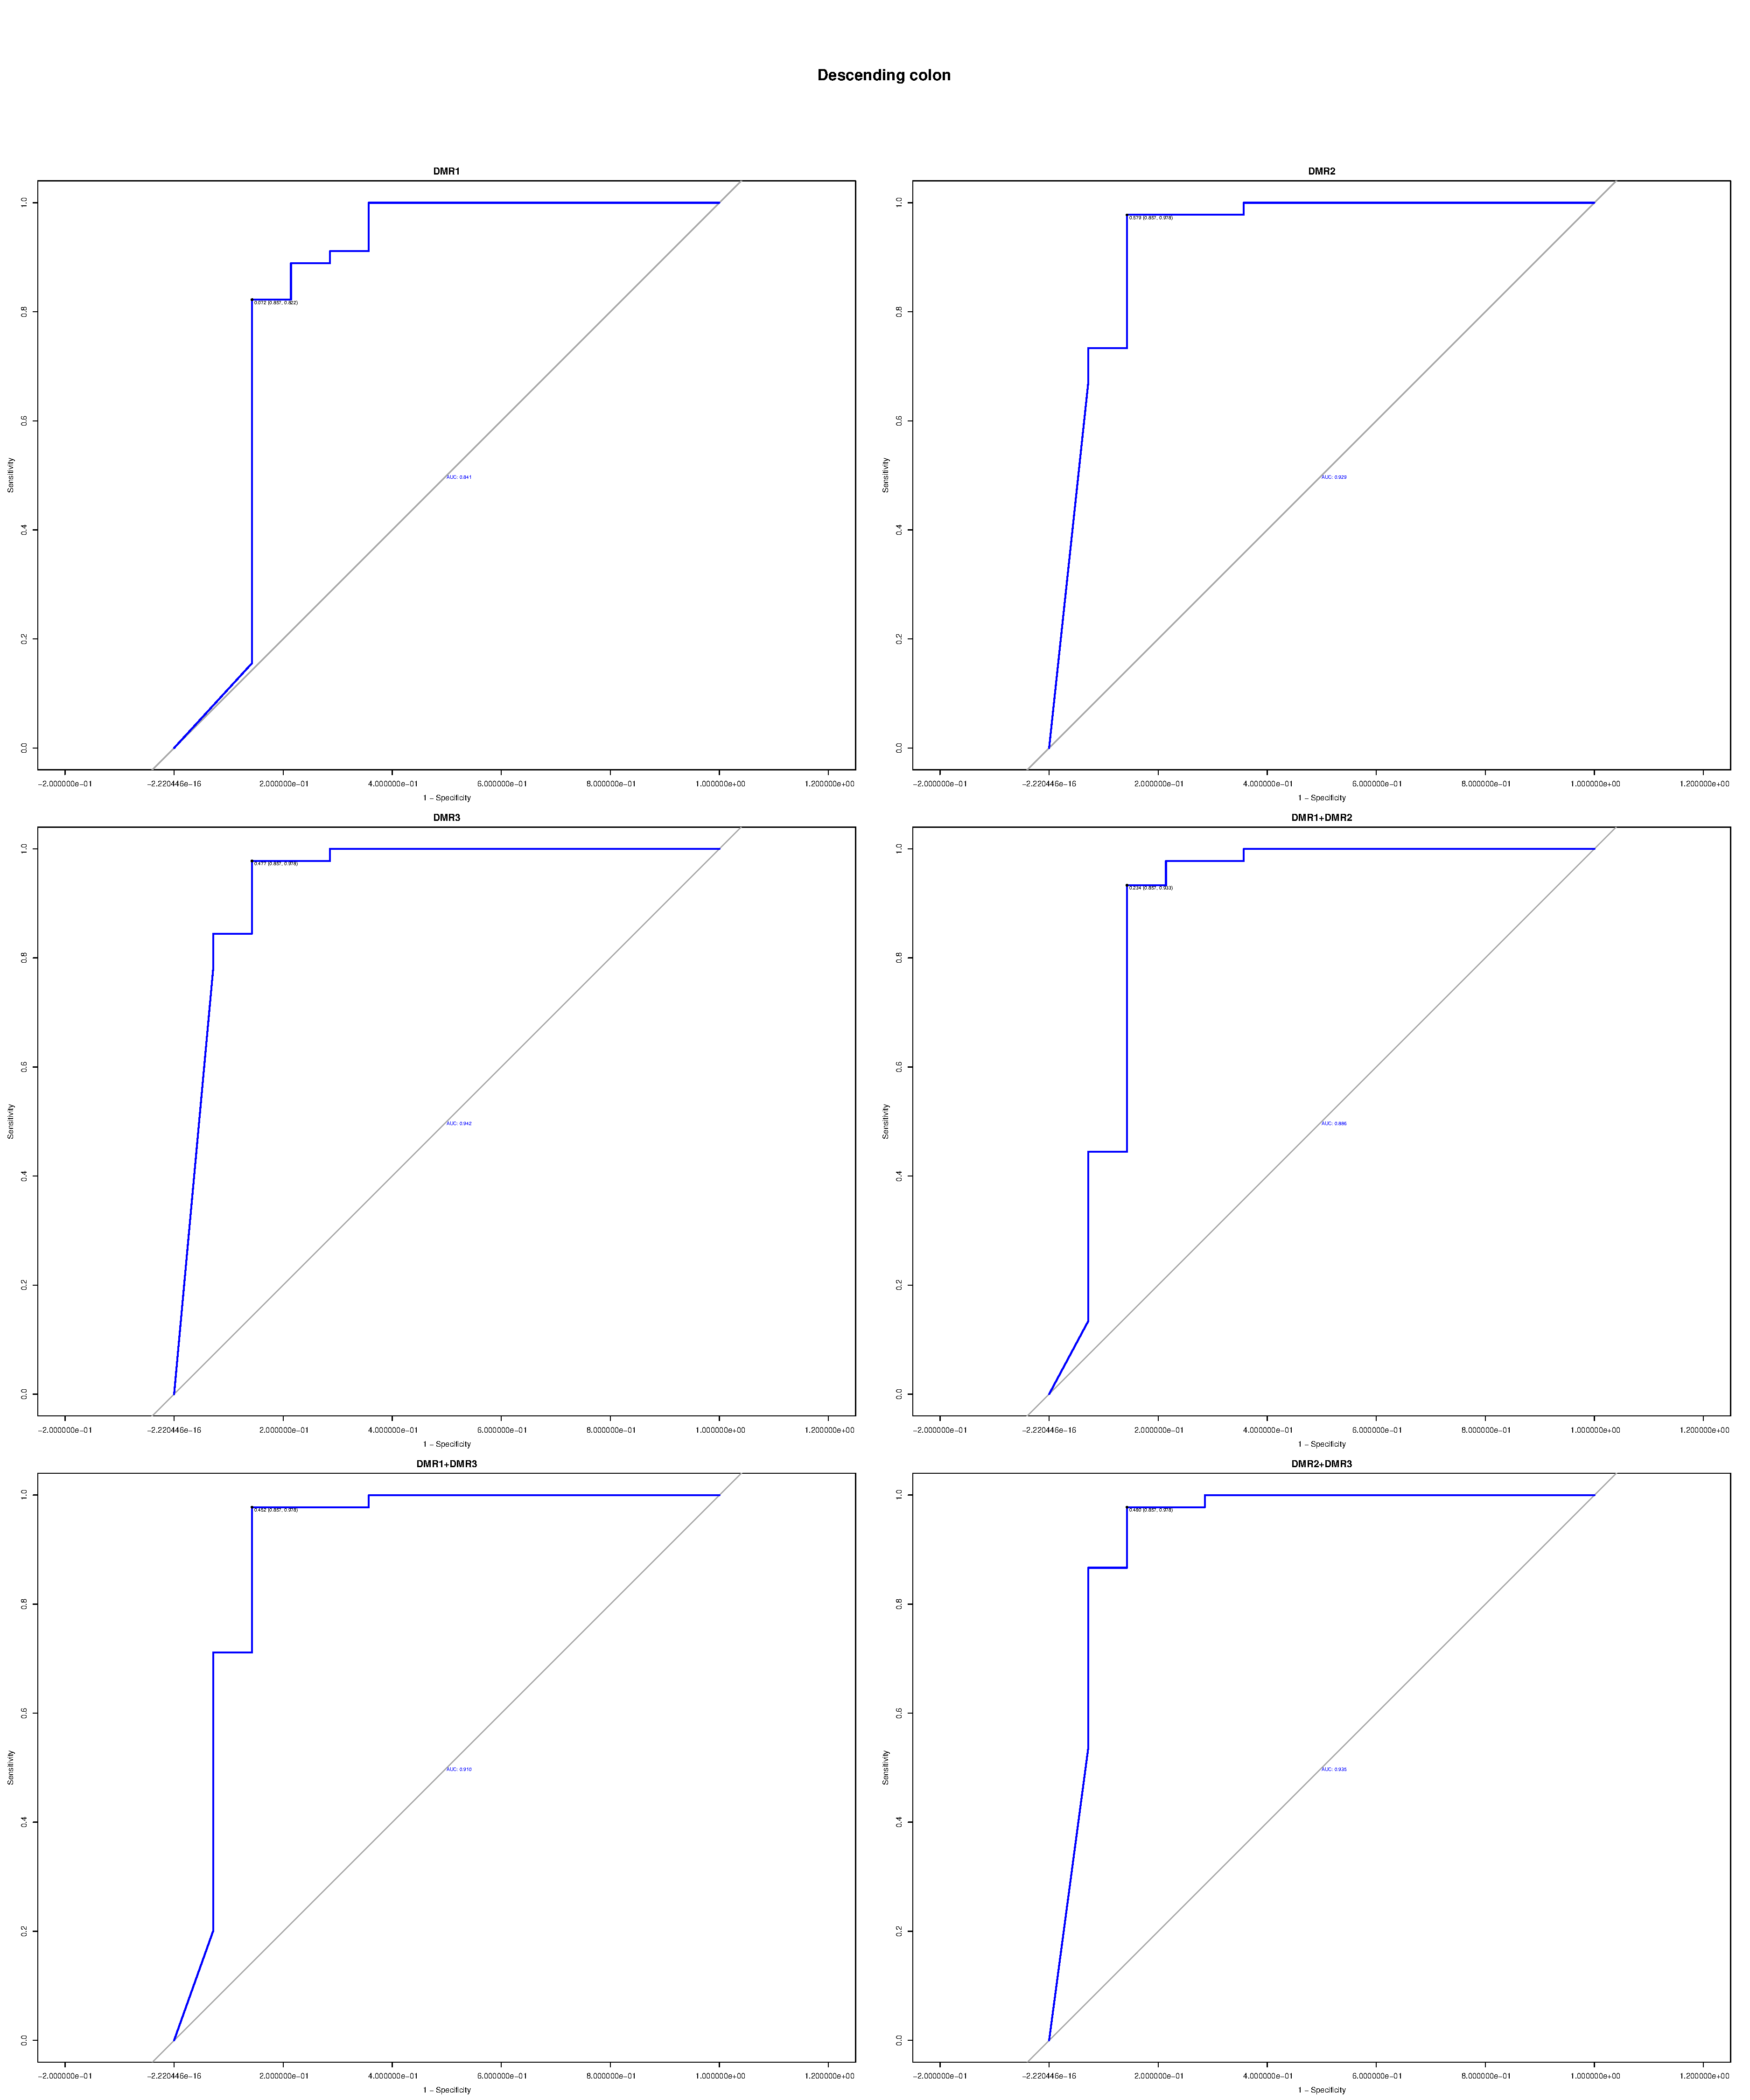
\includegraphics{book1_files/figure-latex/plots-7.pdf}
Hepatic flexure of
colon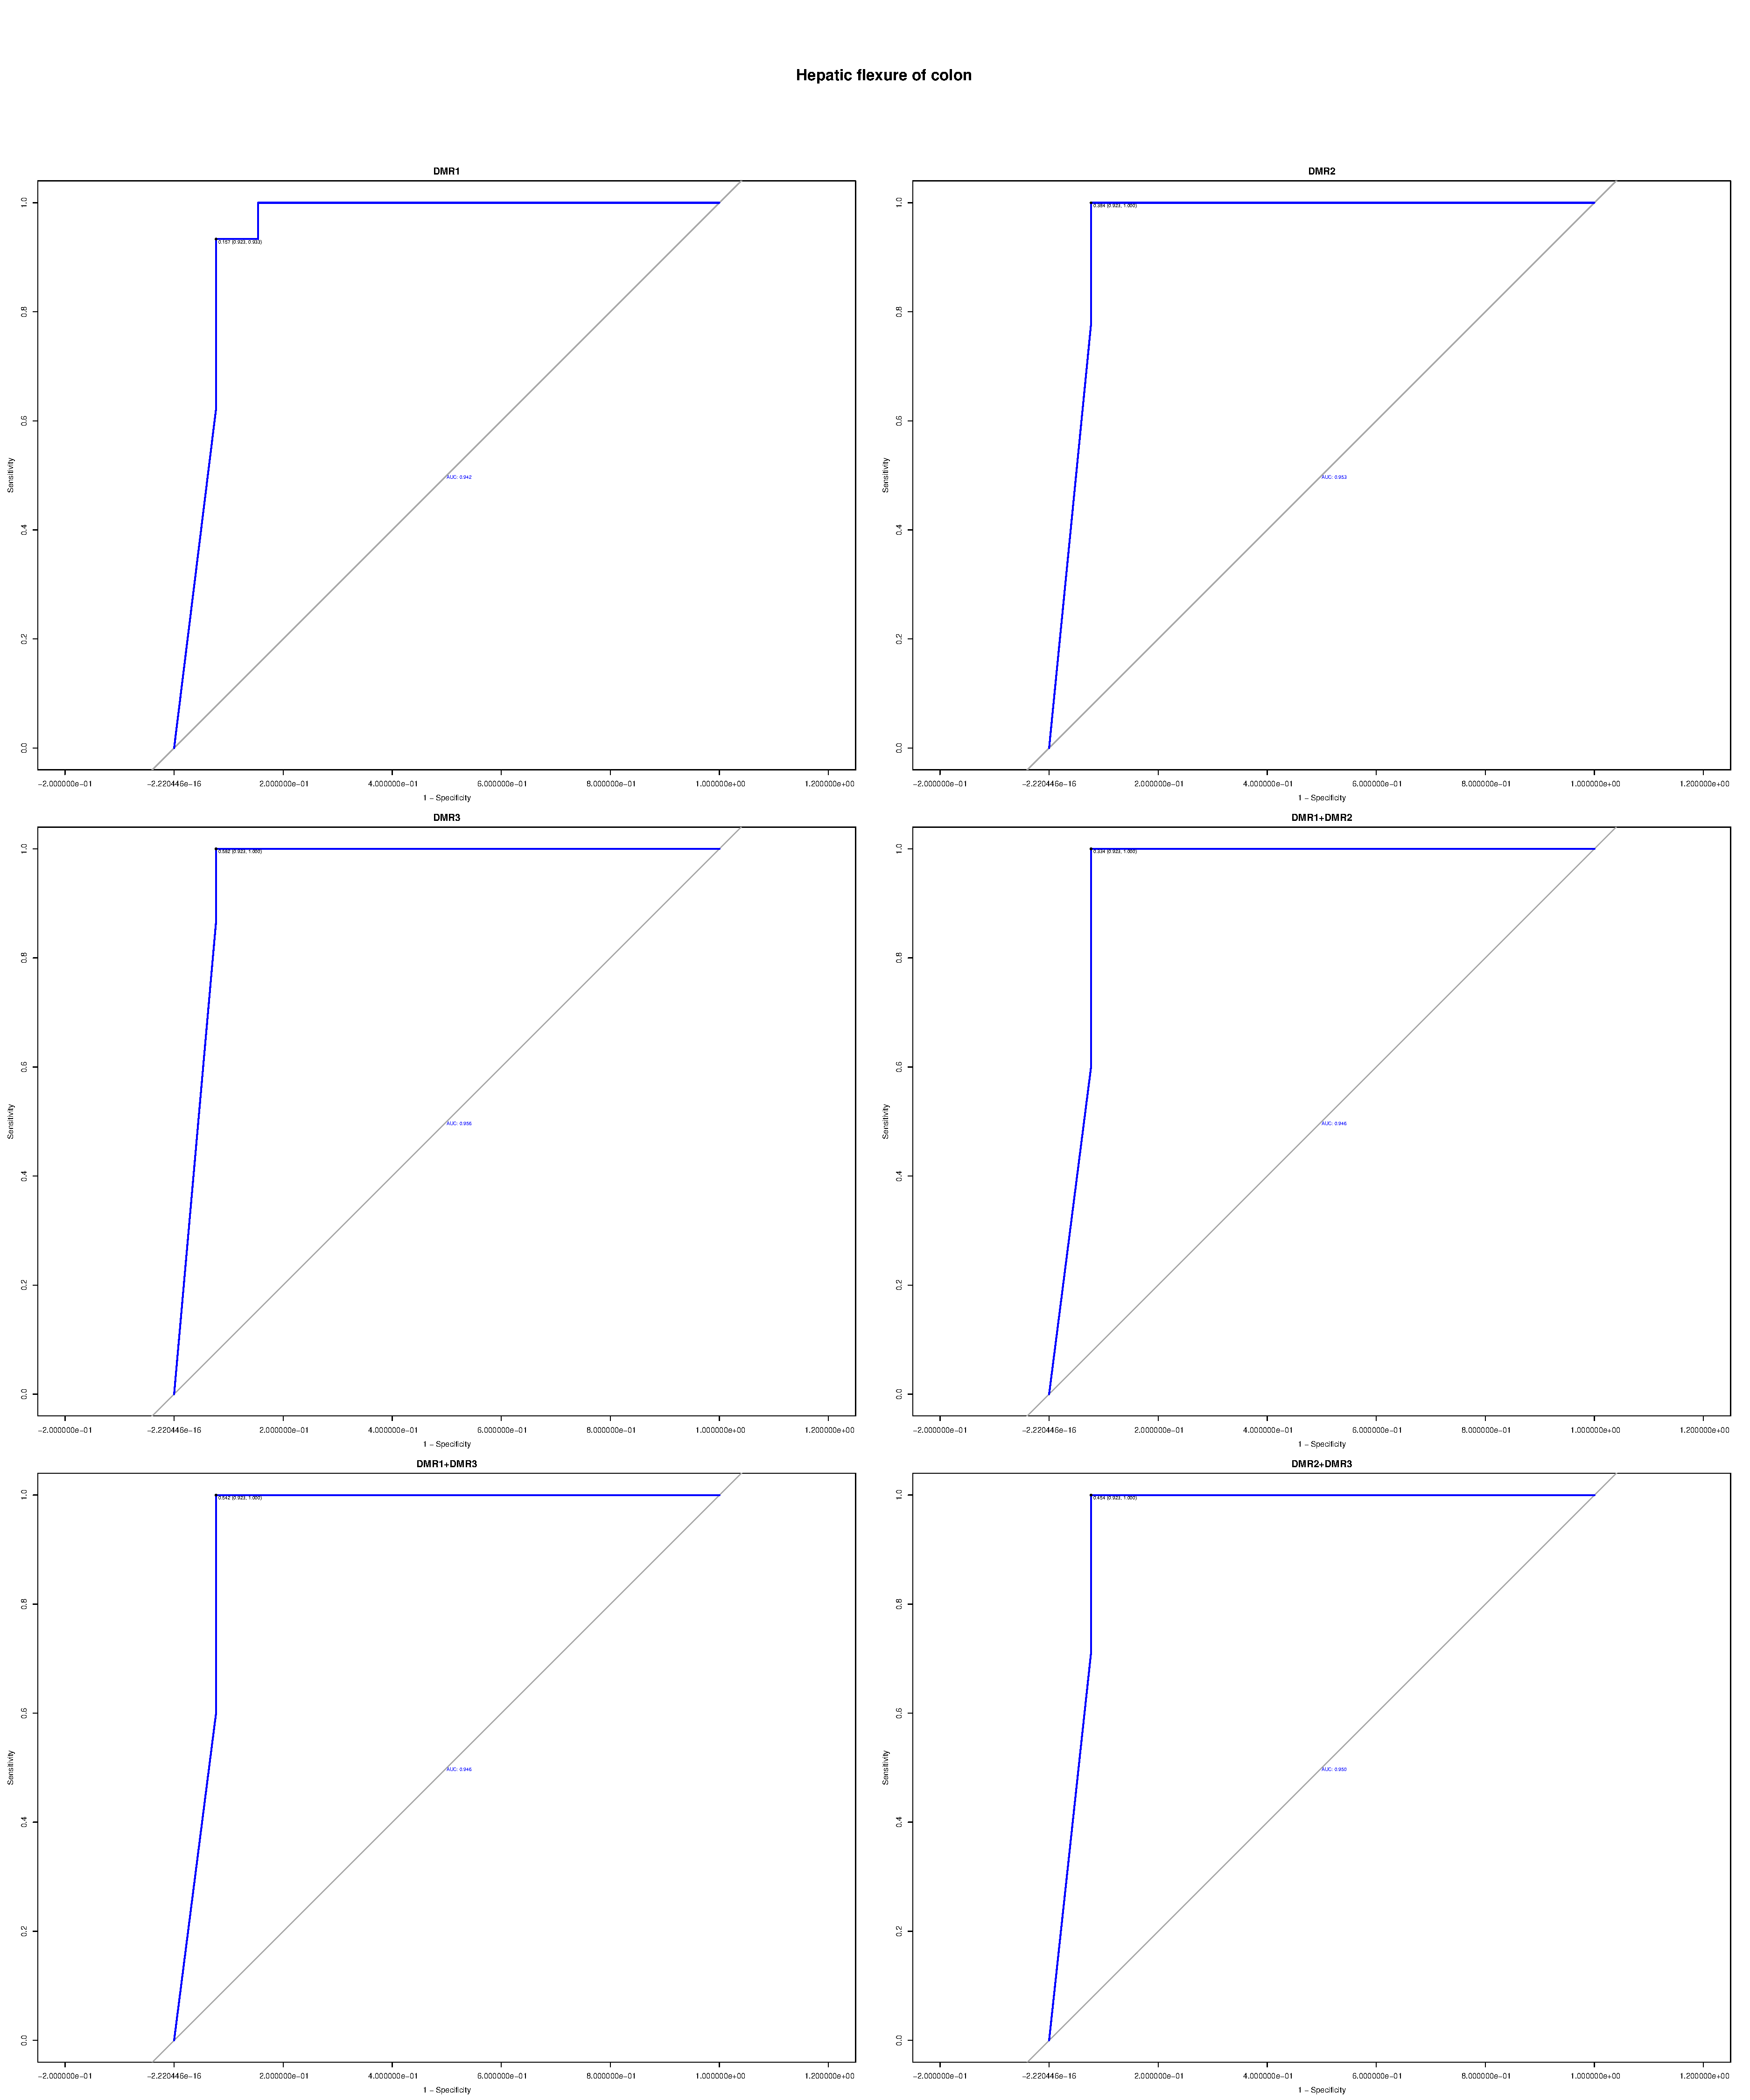
\includegraphics{book1_files/figure-latex/plots-8.pdf} Transverse
colon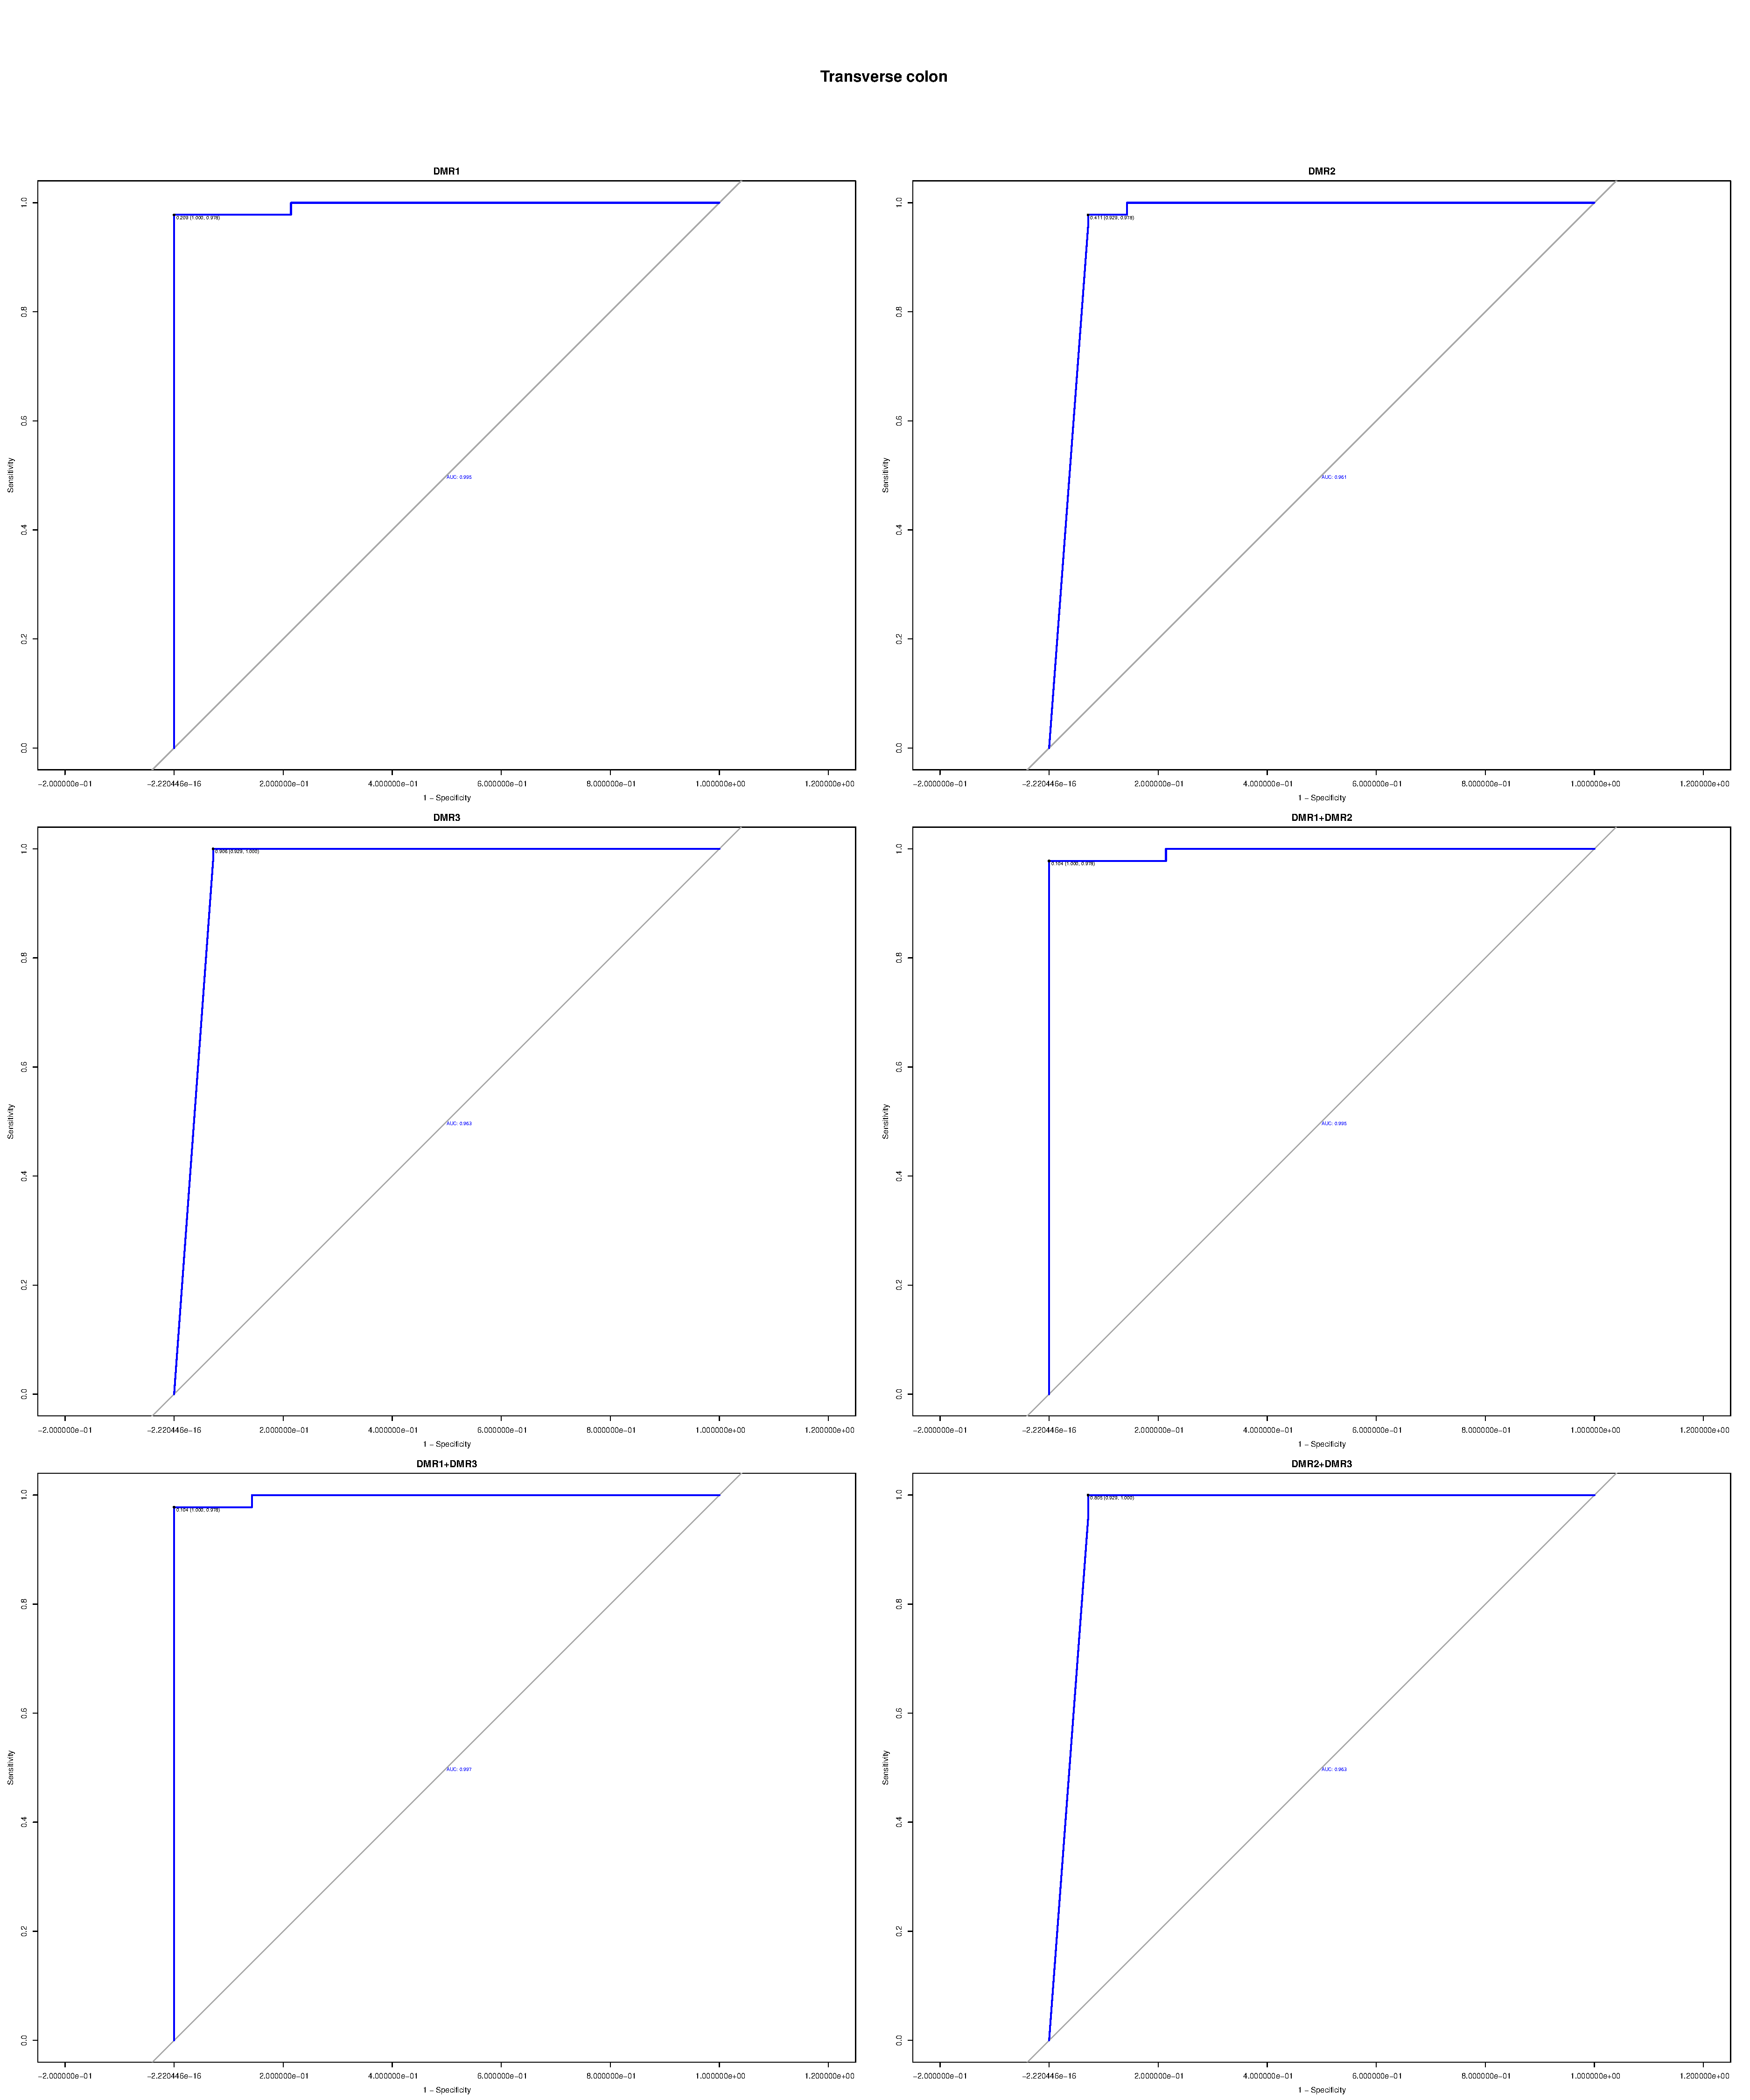
\includegraphics{book1_files/figure-latex/plots-9.pdf} Splenic
flexure of colon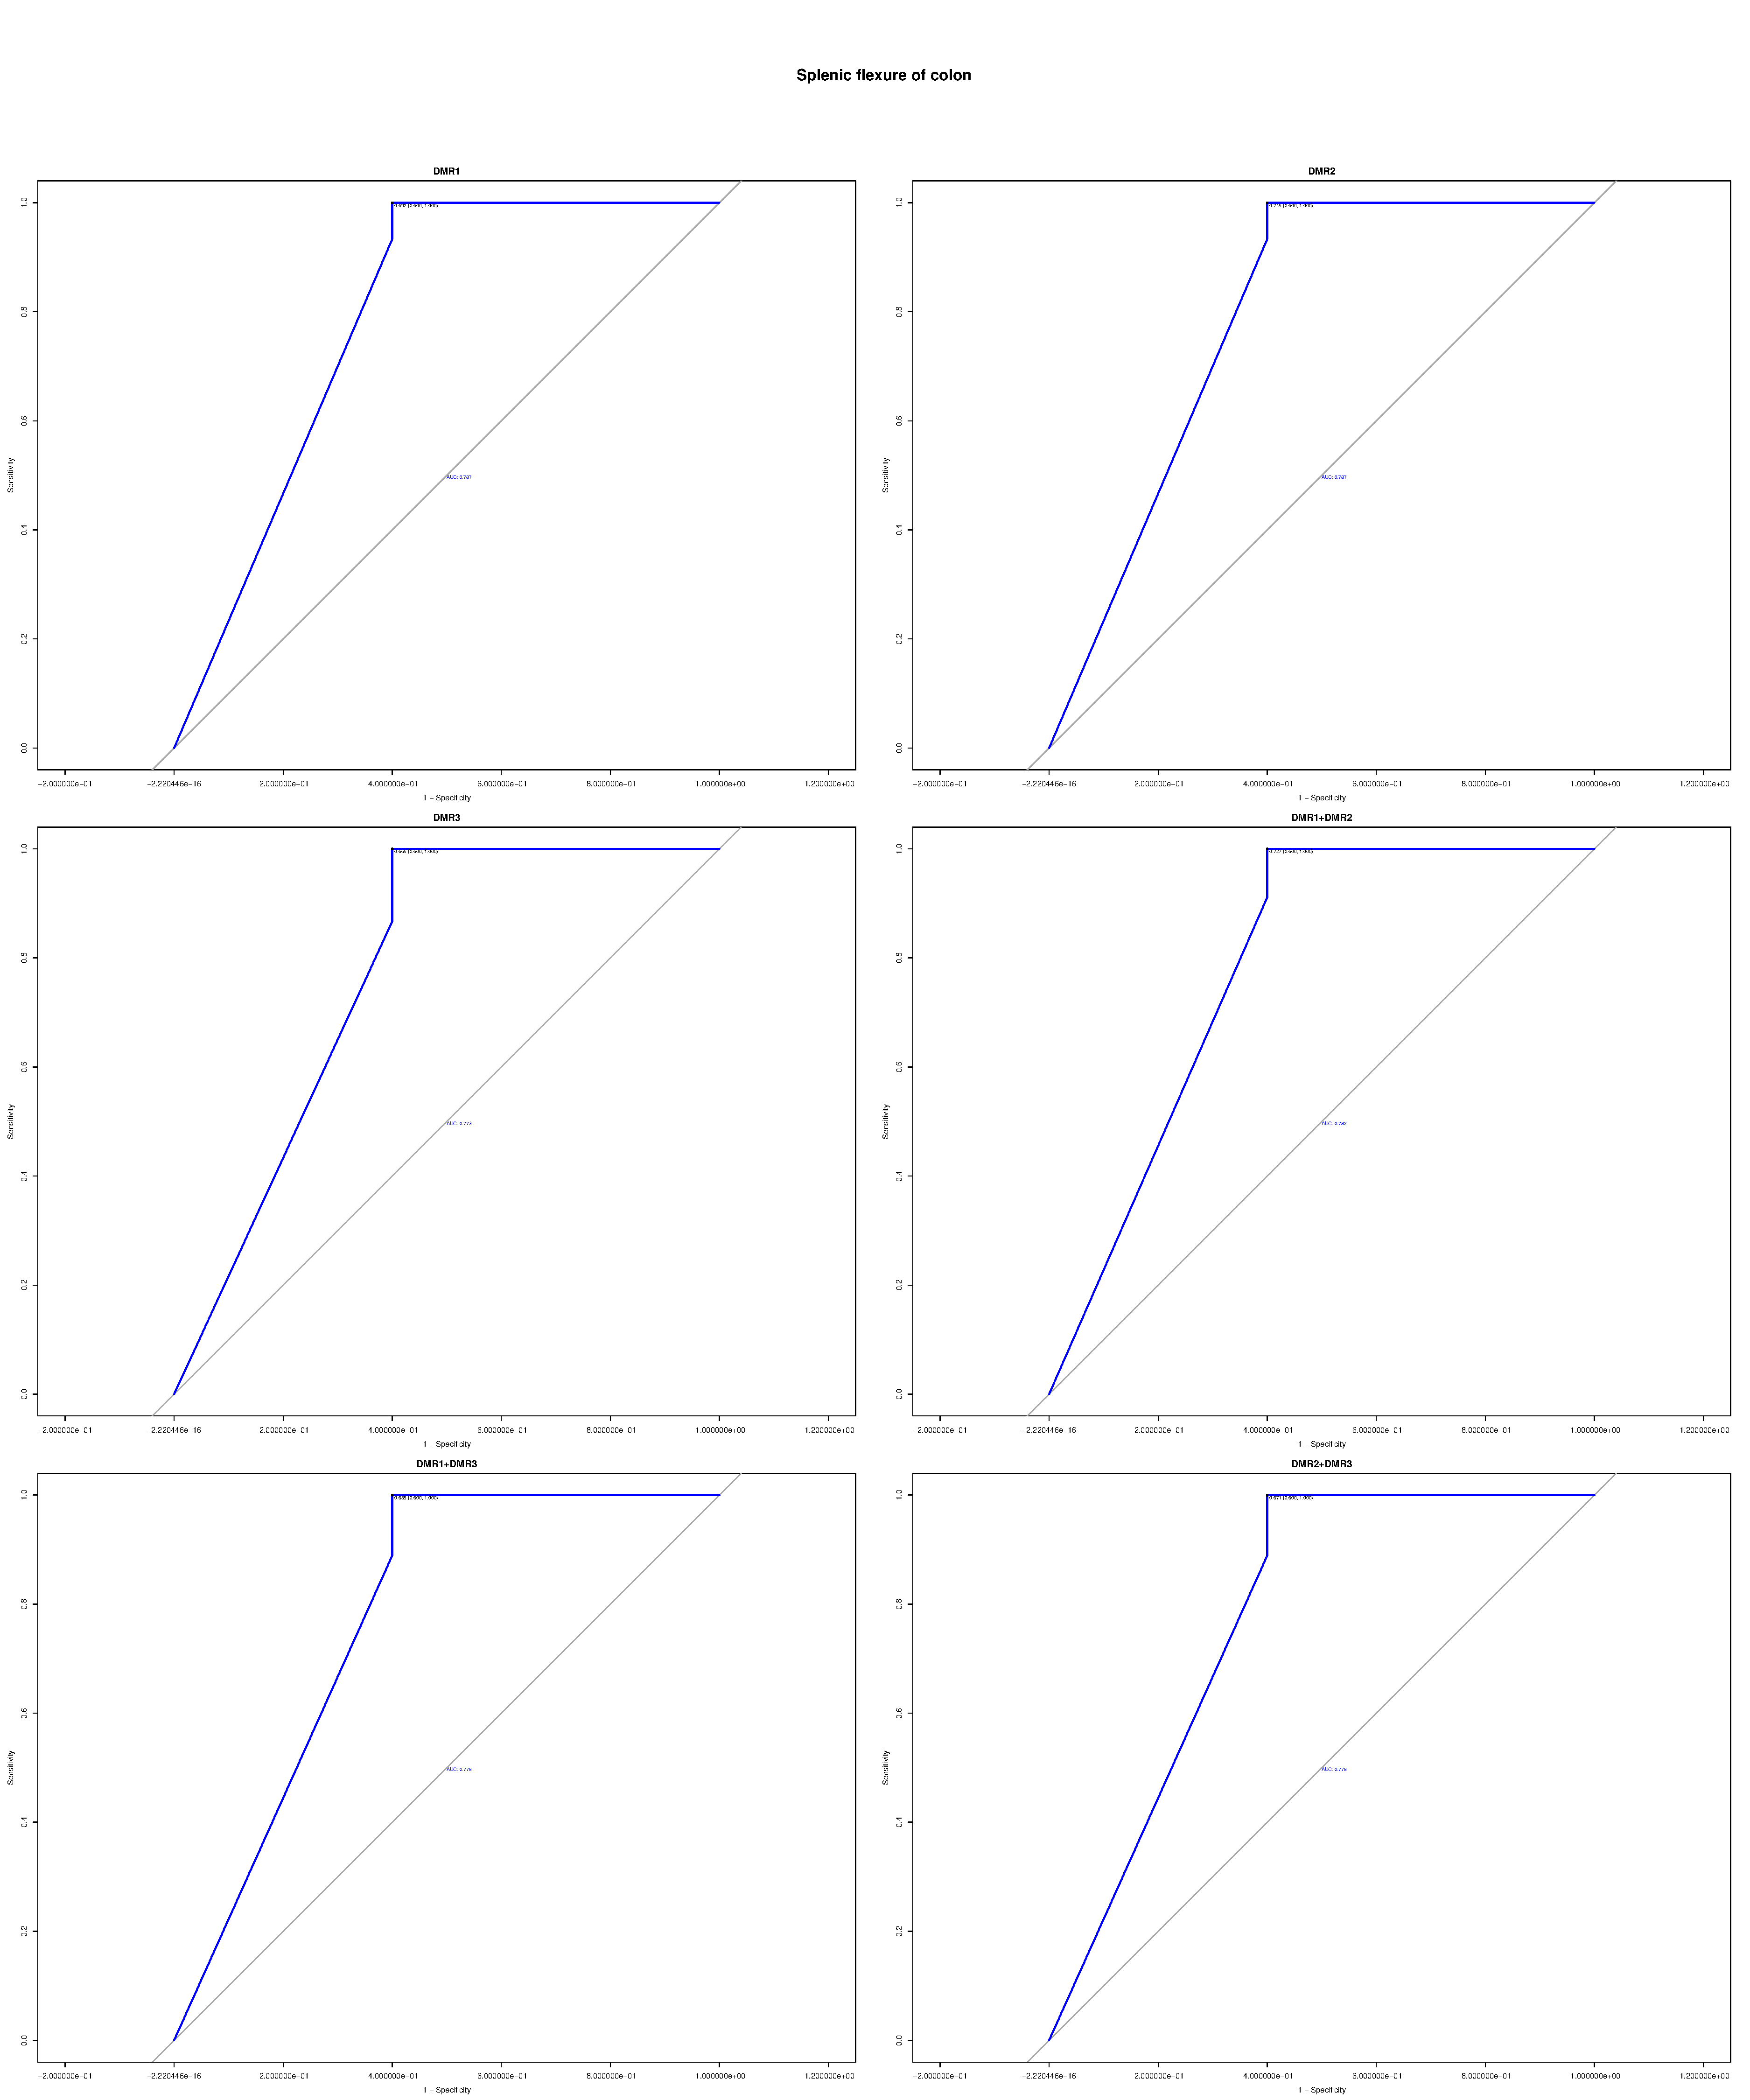
\includegraphics{book1_files/figure-latex/plots-10.pdf}
--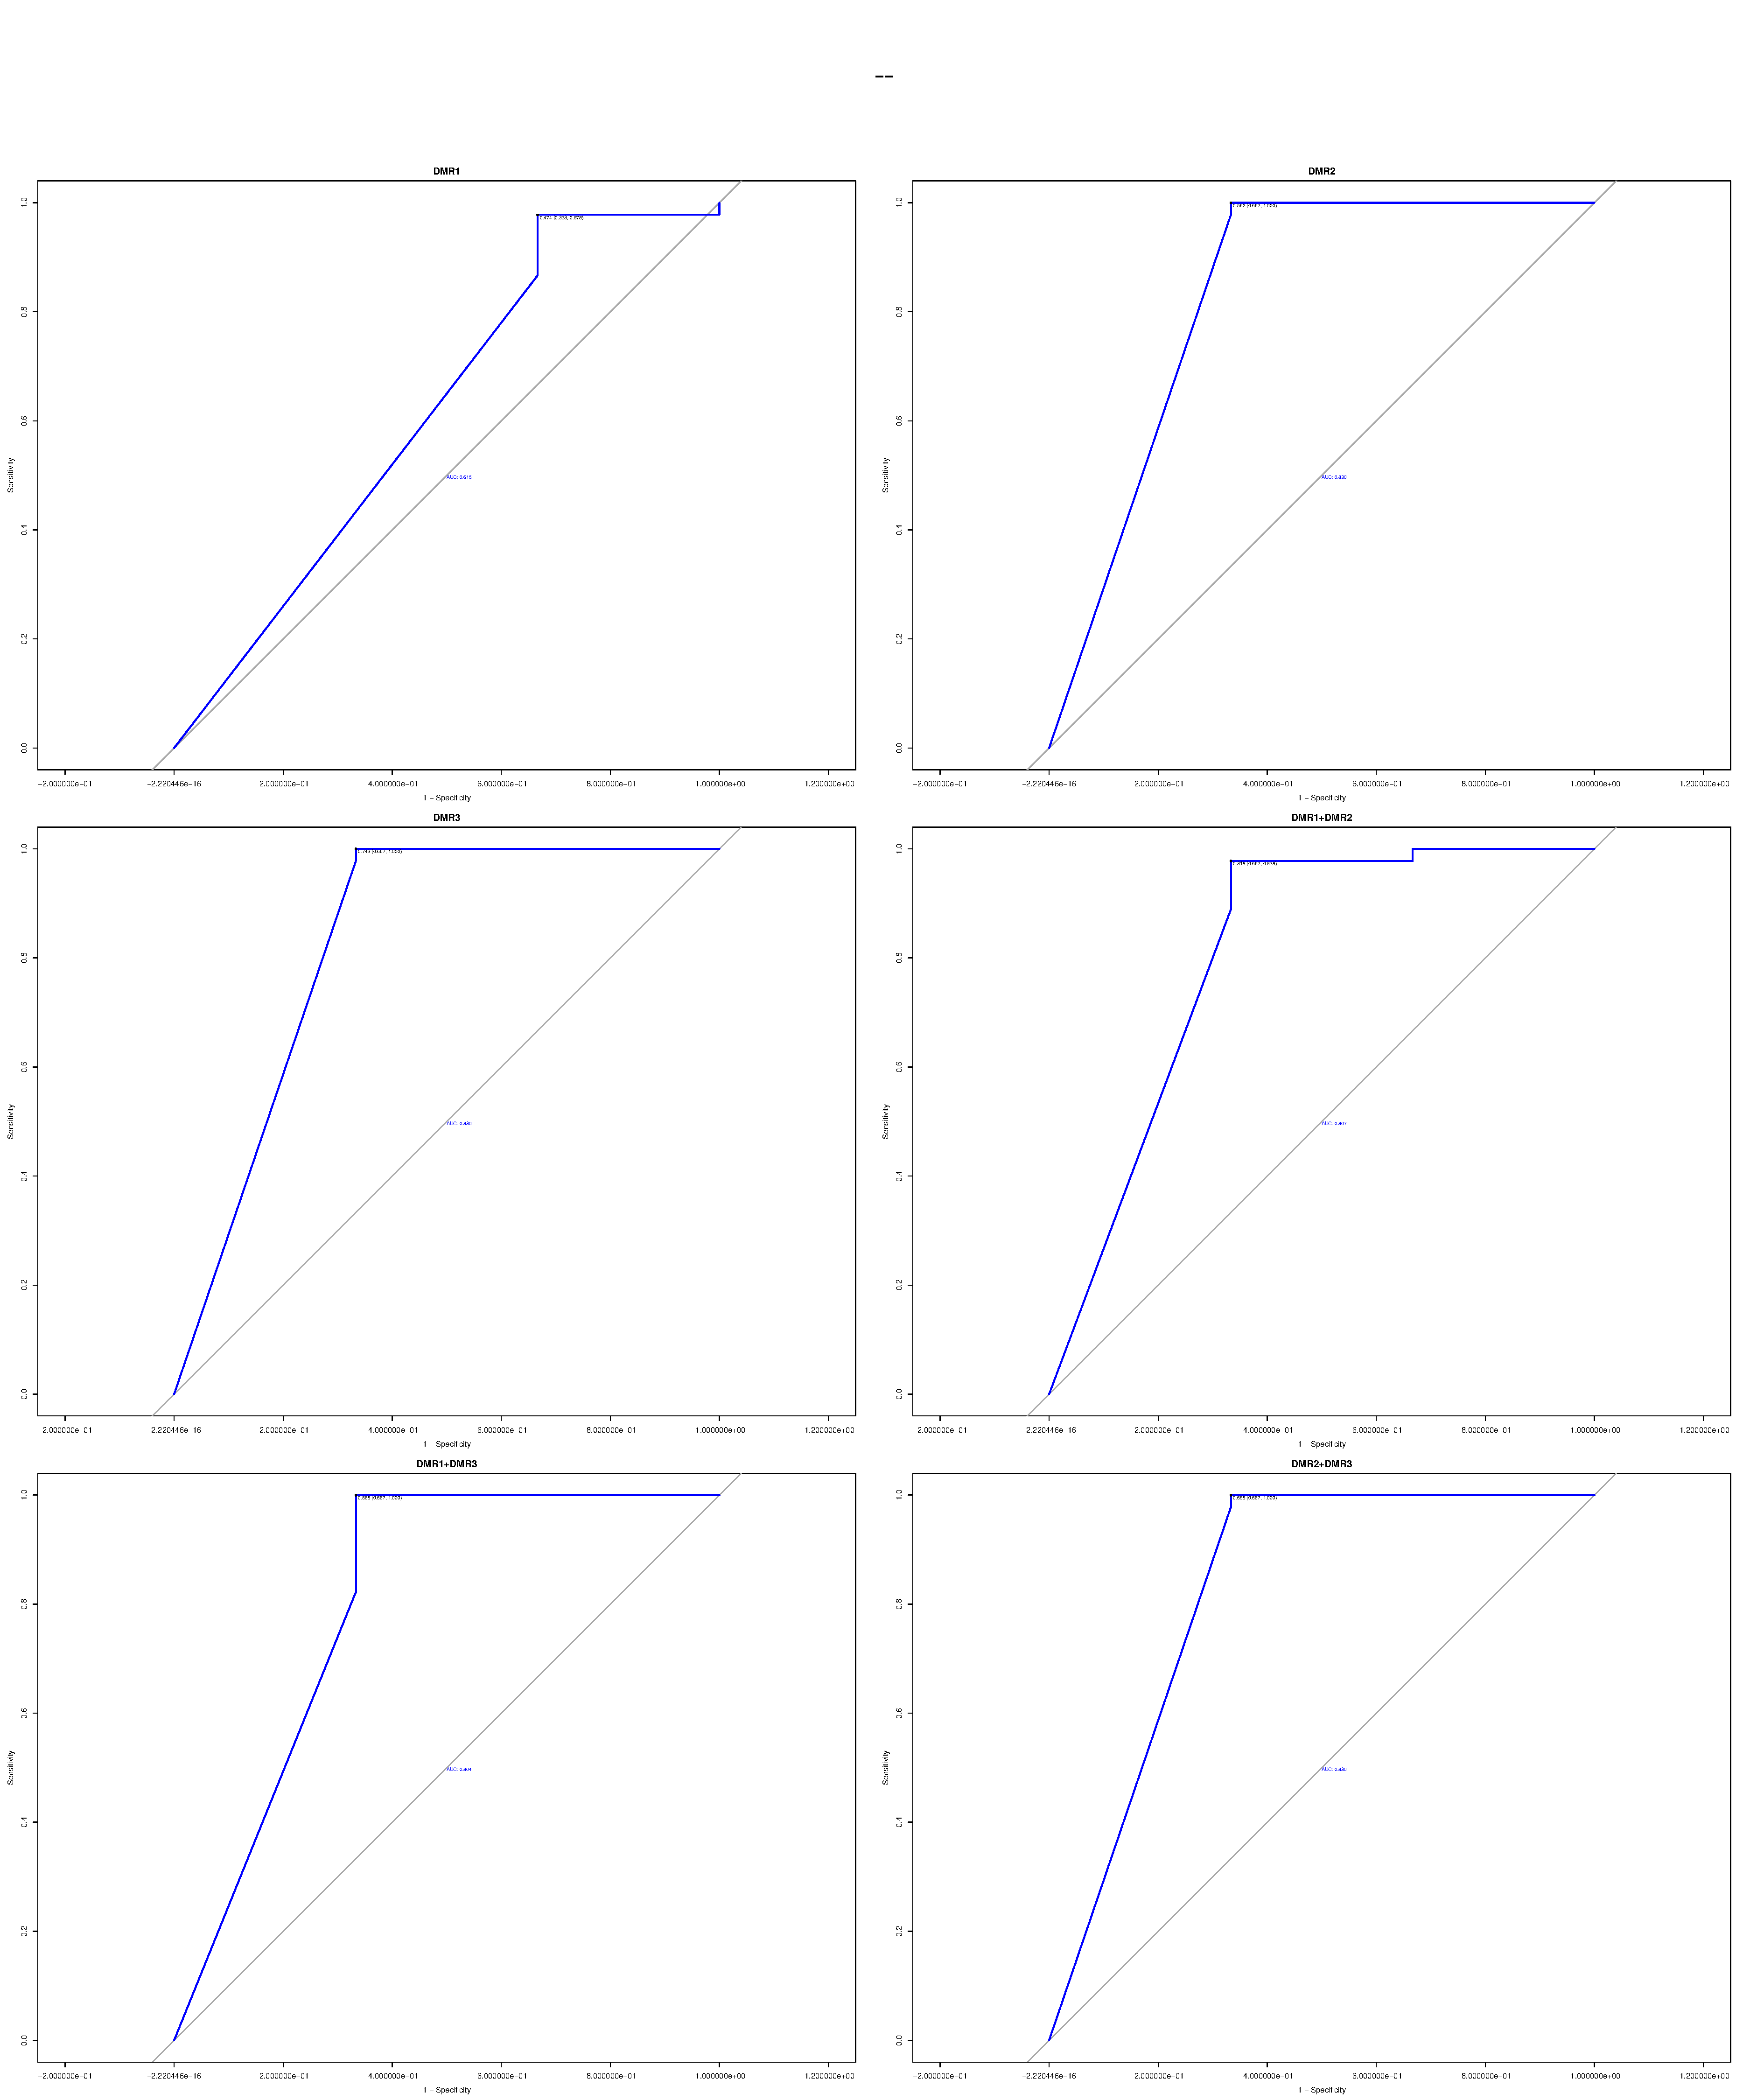
\includegraphics{book1_files/figure-latex/plots-11.pdf} Connective,
subcutaneous and other soft tissues of
abdomen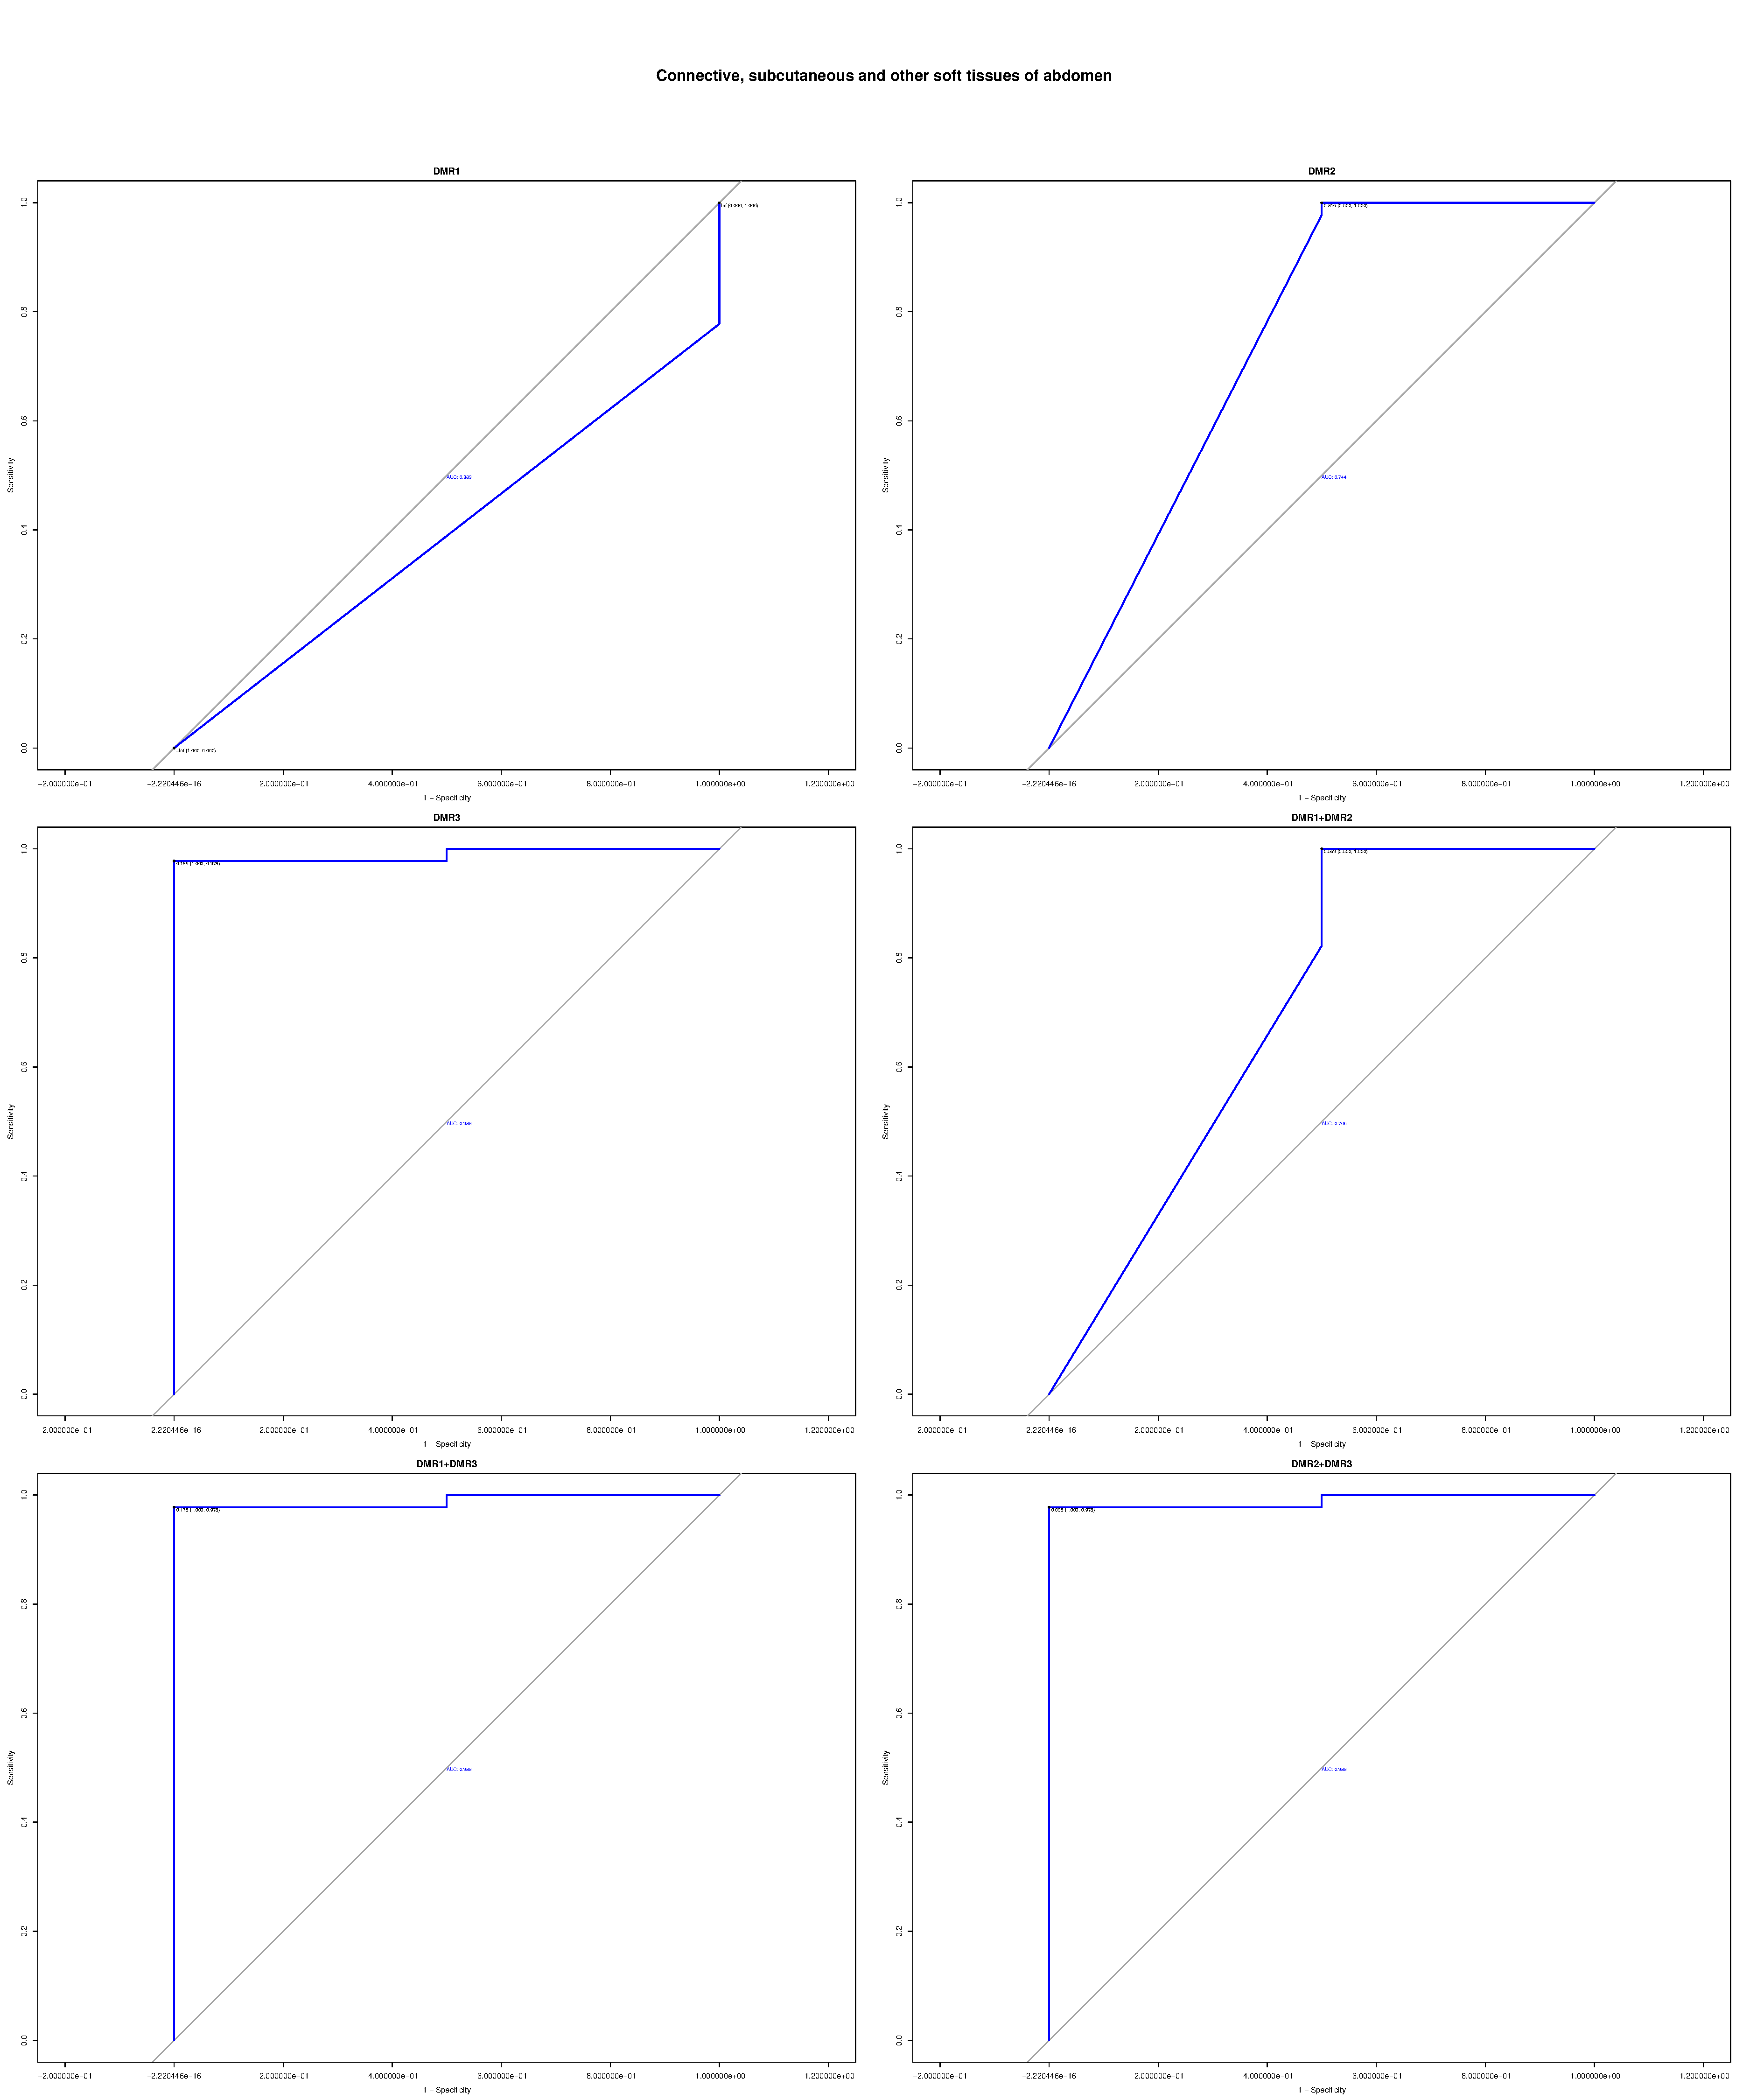
\includegraphics{book1_files/figure-latex/plots-12.pdf}

\bibliography{book.bib,packages.bib}


\end{document}
